\documentclass[english,12pt,a4paper]{article}
\usepackage[T1]{fontenc}
\usepackage{graphicx}
\usepackage{amssymb}
\usepackage{xcolor}
\usepackage{babel}
\usepackage{hyperref}
\usepackage[biber]{biblatex}
\usepackage{siunitx}
\usepackage[breakable]{tcolorbox}
\usepackage{parskip} % Stop auto-indenting (to mimic markdown behaviour)


% Basic figure setup, for now with no caption control since it's done
% automatically by Pandoc (which extracts ![](path) syntax from Markdown).
\usepackage{graphicx}
% Maintain compatibility with old templates. Remove in nbconvert 6.0
\let\Oldincludegraphics\includegraphics
% Ensure that by default, figures have no caption (until we provide a
% proper Figure object with a Caption API and a way to capture that
% in the conversion process - todo).
\usepackage{caption}
\DeclareCaptionFormat{nocaption}{}
\captionsetup{format=nocaption,aboveskip=0pt,belowskip=0pt}

\usepackage{float}
\floatplacement{figure}{H} % forces figures to be placed at the correct location
\usepackage{xcolor} % Allow colors to be defined
\usepackage{enumerate} % Needed for markdown enumerations to work
\usepackage{geometry} % Used to adjust the document margins
\usepackage{amsmath} % Equations
\usepackage{amssymb} % Equations
\usepackage{textcomp} % defines textquotesingle
% Hack from http://tex.stackexchange.com/a/47451/13684:
\AtBeginDocument{%
	\def\PYZsq{\textquotesingle}% Upright quotes in Pygmentized code
}
\usepackage{upquote} % Upright quotes for verbatim code
\usepackage{eurosym} % defines \euro

\usepackage{iftex}
\ifPDFTeX
\usepackage[T1]{fontenc}
\IfFileExists{alphabeta.sty}{
	\usepackage{alphabeta}
}{
	\usepackage[mathletters]{ucs}
	\usepackage[utf8x]{inputenc}
}
\else
\usepackage{fontspec}
\usepackage{unicode-math}
\fi

\usepackage{fancyvrb} % verbatim replacement that allows latex
\usepackage{grffile} % extends the file name processing of package graphics
% to support a larger range
\makeatletter % fix for old versions of grffile with XeLaTeX
\@ifpackagelater{grffile}{2019/11/01}
{
	% Do nothing on new versions
}
{
	\def\Gread@@xetex#1{%
		\IfFileExists{"\Gin@base".bb}%
		{\Gread@eps{\Gin@base.bb}}%
		{\Gread@@xetex@aux#1}%
	}
}
\makeatother
\usepackage[Export]{adjustbox} % Used to constrain images to a maximum size
\adjustboxset{max size={0.9\linewidth}{0.9\paperheight}}

% The hyperref package gives us a pdf with properly built
% internal navigation ('pdf bookmarks' for the table of contents,
% internal cross-reference links, web links for URLs, etc.)
\usepackage{hyperref}
% The default LaTeX title has an obnoxious amount of whitespace. By default,
% titling removes some of it. It also provides customization options.
\usepackage{titling}
\usepackage{longtable} % longtable support required by pandoc >1.10
\usepackage{booktabs}  % table support for pandoc > 1.12.2
\usepackage{array}     % table support for pandoc >= 2.11.3
\usepackage{calc}      % table minipage width calculation for pandoc >= 2.11.1
\usepackage[inline]{enumitem} % IRkernel/repr support (it uses the enumerate* environment)
\usepackage[normalem]{ulem} % ulem is needed to support strikethroughs (\sout)
% normalem makes italics be italics, not underlines
\usepackage{mathrsfs}



% Colors for the hyperref package
\definecolor{urlcolor}{rgb}{0,.145,.698}
\definecolor{linkcolor}{rgb}{.71,0.21,0.01}
\definecolor{citecolor}{rgb}{.12,.54,.11}

% ANSI colors
\definecolor{ansi-black}{HTML}{3E424D}
\definecolor{ansi-black-intense}{HTML}{282C36}
\definecolor{ansi-red}{HTML}{E75C58}
\definecolor{ansi-red-intense}{HTML}{B22B31}
\definecolor{ansi-green}{HTML}{00A250}
\definecolor{ansi-green-intense}{HTML}{007427}
\definecolor{ansi-yellow}{HTML}{DDB62B}
\definecolor{ansi-yellow-intense}{HTML}{B27D12}
\definecolor{ansi-blue}{HTML}{208FFB}
\definecolor{ansi-blue-intense}{HTML}{0065CA}
\definecolor{ansi-magenta}{HTML}{D160C4}
\definecolor{ansi-magenta-intense}{HTML}{A03196}
\definecolor{ansi-cyan}{HTML}{60C6C8}
\definecolor{ansi-cyan-intense}{HTML}{258F8F}
\definecolor{ansi-white}{HTML}{C5C1B4}
\definecolor{ansi-white-intense}{HTML}{A1A6B2}
\definecolor{ansi-default-inverse-fg}{HTML}{FFFFFF}
\definecolor{ansi-default-inverse-bg}{HTML}{000000}

% common color for the border for error outputs.
\definecolor{outerrorbackground}{HTML}{FFDFDF}

% commands and environments needed by pandoc snippets
% extracted from the output of `pandoc -s`
\providecommand{\tightlist}{%
	\setlength{\itemsep}{0pt}\setlength{\parskip}{0pt}}
\DefineVerbatimEnvironment{Highlighting}{Verbatim}{commandchars=\\\{\}}
% Add ',fontsize=\small' for more characters per line
\newenvironment{Shaded}{}{}
\newcommand{\KeywordTok}[1]{\textcolor[rgb]{0.00,0.44,0.13}{\textbf{{#1}}}}
\newcommand{\DataTypeTok}[1]{\textcolor[rgb]{0.56,0.13,0.00}{{#1}}}
\newcommand{\DecValTok}[1]{\textcolor[rgb]{0.25,0.63,0.44}{{#1}}}
\newcommand{\BaseNTok}[1]{\textcolor[rgb]{0.25,0.63,0.44}{{#1}}}
\newcommand{\FloatTok}[1]{\textcolor[rgb]{0.25,0.63,0.44}{{#1}}}
\newcommand{\CharTok}[1]{\textcolor[rgb]{0.25,0.44,0.63}{{#1}}}
\newcommand{\StringTok}[1]{\textcolor[rgb]{0.25,0.44,0.63}{{#1}}}
\newcommand{\CommentTok}[1]{\textcolor[rgb]{0.38,0.63,0.69}{\textit{{#1}}}}
\newcommand{\OtherTok}[1]{\textcolor[rgb]{0.00,0.44,0.13}{{#1}}}
\newcommand{\AlertTok}[1]{\textcolor[rgb]{1.00,0.00,0.00}{\textbf{{#1}}}}
\newcommand{\FunctionTok}[1]{\textcolor[rgb]{0.02,0.16,0.49}{{#1}}}
\newcommand{\RegionMarkerTok}[1]{{#1}}
\newcommand{\ErrorTok}[1]{\textcolor[rgb]{1.00,0.00,0.00}{\textbf{{#1}}}}
\newcommand{\NormalTok}[1]{{#1}}

% Additional commands for more recent versions of Pandoc
\newcommand{\ConstantTok}[1]{\textcolor[rgb]{0.53,0.00,0.00}{{#1}}}
\newcommand{\SpecialCharTok}[1]{\textcolor[rgb]{0.25,0.44,0.63}{{#1}}}
\newcommand{\VerbatimStringTok}[1]{\textcolor[rgb]{0.25,0.44,0.63}{{#1}}}
\newcommand{\SpecialStringTok}[1]{\textcolor[rgb]{0.73,0.40,0.53}{{#1}}}
\newcommand{\ImportTok}[1]{{#1}}
\newcommand{\DocumentationTok}[1]{\textcolor[rgb]{0.73,0.13,0.13}{\textit{{#1}}}}
\newcommand{\AnnotationTok}[1]{\textcolor[rgb]{0.38,0.63,0.69}{\textbf{\textit{{#1}}}}}
\newcommand{\CommentVarTok}[1]{\textcolor[rgb]{0.38,0.63,0.69}{\textbf{\textit{{#1}}}}}
\newcommand{\VariableTok}[1]{\textcolor[rgb]{0.10,0.09,0.49}{{#1}}}
\newcommand{\ControlFlowTok}[1]{\textcolor[rgb]{0.00,0.44,0.13}{\textbf{{#1}}}}
\newcommand{\OperatorTok}[1]{\textcolor[rgb]{0.40,0.40,0.40}{{#1}}}
\newcommand{\BuiltInTok}[1]{{#1}}
\newcommand{\ExtensionTok}[1]{{#1}}
\newcommand{\PreprocessorTok}[1]{\textcolor[rgb]{0.74,0.48,0.00}{{#1}}}
\newcommand{\AttributeTok}[1]{\textcolor[rgb]{0.49,0.56,0.16}{{#1}}}
\newcommand{\InformationTok}[1]{\textcolor[rgb]{0.38,0.63,0.69}{\textbf{\textit{{#1}}}}}
\newcommand{\WarningTok}[1]{\textcolor[rgb]{0.38,0.63,0.69}{\textbf{\textit{{#1}}}}}


% Define a nice break command that doesn't care if a line doesn't already
% exist.
\def\br{\hspace*{\fill} \\* }
% Math Jax compatibility definitions
\def\gt{>}
\def\lt{<}
\let\Oldtex\TeX
\let\Oldlatex\LaTeX
\renewcommand{\TeX}{\textrm{\Oldtex}}
\renewcommand{\LaTeX}{\textrm{\Oldlatex}}
% Document parameters
% Document title
\title{analysis}







% Pygments definitions
\makeatletter
\def\PY@reset{\let\PY@it=\relax \let\PY@bf=\relax%
	\let\PY@ul=\relax \let\PY@tc=\relax%
	\let\PY@bc=\relax \let\PY@ff=\relax}
\def\PY@tok#1{\csname PY@tok@#1\endcsname}
\def\PY@toks#1+{\ifx\relax#1\empty\else%
	\PY@tok{#1}\expandafter\PY@toks\fi}
\def\PY@do#1{\PY@bc{\PY@tc{\PY@ul{%
				\PY@it{\PY@bf{\PY@ff{#1}}}}}}}
\def\PY#1#2{\PY@reset\PY@toks#1+\relax+\PY@do{#2}}

\@namedef{PY@tok@w}{\def\PY@tc##1{\textcolor[rgb]{0.73,0.73,0.73}{##1}}}
\@namedef{PY@tok@c}{\let\PY@it=\textit\def\PY@tc##1{\textcolor[rgb]{0.24,0.48,0.48}{##1}}}
\@namedef{PY@tok@cp}{\def\PY@tc##1{\textcolor[rgb]{0.61,0.40,0.00}{##1}}}
\@namedef{PY@tok@k}{\let\PY@bf=\textbf\def\PY@tc##1{\textcolor[rgb]{0.00,0.50,0.00}{##1}}}
\@namedef{PY@tok@kp}{\def\PY@tc##1{\textcolor[rgb]{0.00,0.50,0.00}{##1}}}
\@namedef{PY@tok@kt}{\def\PY@tc##1{\textcolor[rgb]{0.69,0.00,0.25}{##1}}}
\@namedef{PY@tok@o}{\def\PY@tc##1{\textcolor[rgb]{0.40,0.40,0.40}{##1}}}
\@namedef{PY@tok@ow}{\let\PY@bf=\textbf\def\PY@tc##1{\textcolor[rgb]{0.67,0.13,1.00}{##1}}}
\@namedef{PY@tok@nb}{\def\PY@tc##1{\textcolor[rgb]{0.00,0.50,0.00}{##1}}}
\@namedef{PY@tok@nf}{\def\PY@tc##1{\textcolor[rgb]{0.00,0.00,1.00}{##1}}}
\@namedef{PY@tok@nc}{\let\PY@bf=\textbf\def\PY@tc##1{\textcolor[rgb]{0.00,0.00,1.00}{##1}}}
\@namedef{PY@tok@nn}{\let\PY@bf=\textbf\def\PY@tc##1{\textcolor[rgb]{0.00,0.00,1.00}{##1}}}
\@namedef{PY@tok@ne}{\let\PY@bf=\textbf\def\PY@tc##1{\textcolor[rgb]{0.80,0.25,0.22}{##1}}}
\@namedef{PY@tok@nv}{\def\PY@tc##1{\textcolor[rgb]{0.10,0.09,0.49}{##1}}}
\@namedef{PY@tok@no}{\def\PY@tc##1{\textcolor[rgb]{0.53,0.00,0.00}{##1}}}
\@namedef{PY@tok@nl}{\def\PY@tc##1{\textcolor[rgb]{0.46,0.46,0.00}{##1}}}
\@namedef{PY@tok@ni}{\let\PY@bf=\textbf\def\PY@tc##1{\textcolor[rgb]{0.44,0.44,0.44}{##1}}}
\@namedef{PY@tok@na}{\def\PY@tc##1{\textcolor[rgb]{0.41,0.47,0.13}{##1}}}
\@namedef{PY@tok@nt}{\let\PY@bf=\textbf\def\PY@tc##1{\textcolor[rgb]{0.00,0.50,0.00}{##1}}}
\@namedef{PY@tok@nd}{\def\PY@tc##1{\textcolor[rgb]{0.67,0.13,1.00}{##1}}}
\@namedef{PY@tok@s}{\def\PY@tc##1{\textcolor[rgb]{0.73,0.13,0.13}{##1}}}
\@namedef{PY@tok@sd}{\let\PY@it=\textit\def\PY@tc##1{\textcolor[rgb]{0.73,0.13,0.13}{##1}}}
\@namedef{PY@tok@si}{\let\PY@bf=\textbf\def\PY@tc##1{\textcolor[rgb]{0.64,0.35,0.47}{##1}}}
\@namedef{PY@tok@se}{\let\PY@bf=\textbf\def\PY@tc##1{\textcolor[rgb]{0.67,0.36,0.12}{##1}}}
\@namedef{PY@tok@sr}{\def\PY@tc##1{\textcolor[rgb]{0.64,0.35,0.47}{##1}}}
\@namedef{PY@tok@ss}{\def\PY@tc##1{\textcolor[rgb]{0.10,0.09,0.49}{##1}}}
\@namedef{PY@tok@sx}{\def\PY@tc##1{\textcolor[rgb]{0.00,0.50,0.00}{##1}}}
\@namedef{PY@tok@m}{\def\PY@tc##1{\textcolor[rgb]{0.40,0.40,0.40}{##1}}}
\@namedef{PY@tok@gh}{\let\PY@bf=\textbf\def\PY@tc##1{\textcolor[rgb]{0.00,0.00,0.50}{##1}}}
\@namedef{PY@tok@gu}{\let\PY@bf=\textbf\def\PY@tc##1{\textcolor[rgb]{0.50,0.00,0.50}{##1}}}
\@namedef{PY@tok@gd}{\def\PY@tc##1{\textcolor[rgb]{0.63,0.00,0.00}{##1}}}
\@namedef{PY@tok@gi}{\def\PY@tc##1{\textcolor[rgb]{0.00,0.52,0.00}{##1}}}
\@namedef{PY@tok@gr}{\def\PY@tc##1{\textcolor[rgb]{0.89,0.00,0.00}{##1}}}
\@namedef{PY@tok@ge}{\let\PY@it=\textit}
\@namedef{PY@tok@gs}{\let\PY@bf=\textbf}
\@namedef{PY@tok@gp}{\let\PY@bf=\textbf\def\PY@tc##1{\textcolor[rgb]{0.00,0.00,0.50}{##1}}}
\@namedef{PY@tok@go}{\def\PY@tc##1{\textcolor[rgb]{0.44,0.44,0.44}{##1}}}
\@namedef{PY@tok@gt}{\def\PY@tc##1{\textcolor[rgb]{0.00,0.27,0.87}{##1}}}
\@namedef{PY@tok@err}{\def\PY@bc##1{{\setlength{\fboxsep}{\string -\fboxrule}\fcolorbox[rgb]{1.00,0.00,0.00}{1,1,1}{\strut ##1}}}}
\@namedef{PY@tok@kc}{\let\PY@bf=\textbf\def\PY@tc##1{\textcolor[rgb]{0.00,0.50,0.00}{##1}}}
\@namedef{PY@tok@kd}{\let\PY@bf=\textbf\def\PY@tc##1{\textcolor[rgb]{0.00,0.50,0.00}{##1}}}
\@namedef{PY@tok@kn}{\let\PY@bf=\textbf\def\PY@tc##1{\textcolor[rgb]{0.00,0.50,0.00}{##1}}}
\@namedef{PY@tok@kr}{\let\PY@bf=\textbf\def\PY@tc##1{\textcolor[rgb]{0.00,0.50,0.00}{##1}}}
\@namedef{PY@tok@bp}{\def\PY@tc##1{\textcolor[rgb]{0.00,0.50,0.00}{##1}}}
\@namedef{PY@tok@fm}{\def\PY@tc##1{\textcolor[rgb]{0.00,0.00,1.00}{##1}}}
\@namedef{PY@tok@vc}{\def\PY@tc##1{\textcolor[rgb]{0.10,0.09,0.49}{##1}}}
\@namedef{PY@tok@vg}{\def\PY@tc##1{\textcolor[rgb]{0.10,0.09,0.49}{##1}}}
\@namedef{PY@tok@vi}{\def\PY@tc##1{\textcolor[rgb]{0.10,0.09,0.49}{##1}}}
\@namedef{PY@tok@vm}{\def\PY@tc##1{\textcolor[rgb]{0.10,0.09,0.49}{##1}}}
\@namedef{PY@tok@sa}{\def\PY@tc##1{\textcolor[rgb]{0.73,0.13,0.13}{##1}}}
\@namedef{PY@tok@sb}{\def\PY@tc##1{\textcolor[rgb]{0.73,0.13,0.13}{##1}}}
\@namedef{PY@tok@sc}{\def\PY@tc##1{\textcolor[rgb]{0.73,0.13,0.13}{##1}}}
\@namedef{PY@tok@dl}{\def\PY@tc##1{\textcolor[rgb]{0.73,0.13,0.13}{##1}}}
\@namedef{PY@tok@s2}{\def\PY@tc##1{\textcolor[rgb]{0.73,0.13,0.13}{##1}}}
\@namedef{PY@tok@sh}{\def\PY@tc##1{\textcolor[rgb]{0.73,0.13,0.13}{##1}}}
\@namedef{PY@tok@s1}{\def\PY@tc##1{\textcolor[rgb]{0.73,0.13,0.13}{##1}}}
\@namedef{PY@tok@mb}{\def\PY@tc##1{\textcolor[rgb]{0.40,0.40,0.40}{##1}}}
\@namedef{PY@tok@mf}{\def\PY@tc##1{\textcolor[rgb]{0.40,0.40,0.40}{##1}}}
\@namedef{PY@tok@mh}{\def\PY@tc##1{\textcolor[rgb]{0.40,0.40,0.40}{##1}}}
\@namedef{PY@tok@mi}{\def\PY@tc##1{\textcolor[rgb]{0.40,0.40,0.40}{##1}}}
\@namedef{PY@tok@il}{\def\PY@tc##1{\textcolor[rgb]{0.40,0.40,0.40}{##1}}}
\@namedef{PY@tok@mo}{\def\PY@tc##1{\textcolor[rgb]{0.40,0.40,0.40}{##1}}}
\@namedef{PY@tok@ch}{\let\PY@it=\textit\def\PY@tc##1{\textcolor[rgb]{0.24,0.48,0.48}{##1}}}
\@namedef{PY@tok@cm}{\let\PY@it=\textit\def\PY@tc##1{\textcolor[rgb]{0.24,0.48,0.48}{##1}}}
\@namedef{PY@tok@cpf}{\let\PY@it=\textit\def\PY@tc##1{\textcolor[rgb]{0.24,0.48,0.48}{##1}}}
\@namedef{PY@tok@c1}{\let\PY@it=\textit\def\PY@tc##1{\textcolor[rgb]{0.24,0.48,0.48}{##1}}}
\@namedef{PY@tok@cs}{\let\PY@it=\textit\def\PY@tc##1{\textcolor[rgb]{0.24,0.48,0.48}{##1}}}

\def\PYZbs{\char`\\}
\def\PYZus{\char`\_}
\def\PYZob{\char`\{}
\def\PYZcb{\char`\}}
\def\PYZca{\char`\^}
\def\PYZam{\char`\&}
\def\PYZlt{\char`\<}
\def\PYZgt{\char`\>}
\def\PYZsh{\char`\#}
\def\PYZpc{\char`\%}
\def\PYZdl{\char`\$}
\def\PYZhy{\char`\-}
\def\PYZsq{\char`\'}
\def\PYZdq{\char`\"}
\def\PYZti{\char`\~}
% for compatibility with earlier versions
\def\PYZat{@}
\def\PYZlb{[}
\def\PYZrb{]}
\makeatother


% For linebreaks inside Verbatim environment from package fancyvrb.
\makeatletter
\newbox\Wrappedcontinuationbox
\newbox\Wrappedvisiblespacebox
\newcommand*\Wrappedvisiblespace {\textcolor{red}{\textvisiblespace}}
\newcommand*\Wrappedcontinuationsymbol {\textcolor{red}{\llap{\tiny$\m@th\hookrightarrow$}}}
\newcommand*\Wrappedcontinuationindent {3ex }
\newcommand*\Wrappedafterbreak {\kern\Wrappedcontinuationindent\copy\Wrappedcontinuationbox}
% Take advantage of the already applied Pygments mark-up to insert
% potential linebreaks for TeX processing.
%        {, <, #, %, $, ' and ": go to next line.
	%        _, }, ^, &, >, - and ~: stay at end of broken line.
% Use of \textquotesingle for straight quote.
\newcommand*\Wrappedbreaksatspecials {%
	\def\PYGZus{\discretionary{\char`\_}{\Wrappedafterbreak}{\char`\_}}%
	\def\PYGZob{\discretionary{}{\Wrappedafterbreak\char`\{}{\char`\{}}%
	\def\PYGZcb{\discretionary{\char`\}}{\Wrappedafterbreak}{\char`\}}}%
	\def\PYGZca{\discretionary{\char`\^}{\Wrappedafterbreak}{\char`\^}}%
	\def\PYGZam{\discretionary{\char`\&}{\Wrappedafterbreak}{\char`\&}}%
	\def\PYGZlt{\discretionary{}{\Wrappedafterbreak\char`\<}{\char`\<}}%
	\def\PYGZgt{\discretionary{\char`\>}{\Wrappedafterbreak}{\char`\>}}%
	\def\PYGZsh{\discretionary{}{\Wrappedafterbreak\char`\#}{\char`\#}}%
	\def\PYGZpc{\discretionary{}{\Wrappedafterbreak\char`\%}{\char`\%}}%
	\def\PYGZdl{\discretionary{}{\Wrappedafterbreak\char`\$}{\char`\$}}%
	\def\PYGZhy{\discretionary{\char`\-}{\Wrappedafterbreak}{\char`\-}}%
	\def\PYGZsq{\discretionary{}{\Wrappedafterbreak\textquotesingle}{\textquotesingle}}%
	\def\PYGZdq{\discretionary{}{\Wrappedafterbreak\char`\"}{\char`\"}}%
	\def\PYGZti{\discretionary{\char`\~}{\Wrappedafterbreak}{\char`\~}}%
}
% Some characters . , ; ? ! / are not pygmentized.
% This macro makes them "active" and they will insert potential linebreaks
\newcommand*\Wrappedbreaksatpunct {%
	\lccode`\~`\.\lowercase{\def~}{\discretionary{\hbox{\char`\.}}{\Wrappedafterbreak}{\hbox{\char`\.}}}%
	\lccode`\~`\,\lowercase{\def~}{\discretionary{\hbox{\char`\,}}{\Wrappedafterbreak}{\hbox{\char`\,}}}%
	\lccode`\~`\;\lowercase{\def~}{\discretionary{\hbox{\char`\;}}{\Wrappedafterbreak}{\hbox{\char`\;}}}%
	\lccode`\~`\:\lowercase{\def~}{\discretionary{\hbox{\char`\:}}{\Wrappedafterbreak}{\hbox{\char`\:}}}%
	\lccode`\~`\?\lowercase{\def~}{\discretionary{\hbox{\char`\?}}{\Wrappedafterbreak}{\hbox{\char`\?}}}%
	\lccode`\~`\!\lowercase{\def~}{\discretionary{\hbox{\char`\!}}{\Wrappedafterbreak}{\hbox{\char`\!}}}%
	\lccode`\~`\/\lowercase{\def~}{\discretionary{\hbox{\char`\/}}{\Wrappedafterbreak}{\hbox{\char`\/}}}%
	\catcode`\.\active
	\catcode`\,\active
	\catcode`\;\active
	\catcode`\:\active
	\catcode`\?\active
	\catcode`\!\active
	\catcode`\/\active
	\lccode`\~`\~
}
\makeatother

\let\OriginalVerbatim=\Verbatim
\makeatletter
\renewcommand{\Verbatim}[1][1]{%
	%\parskip\z@skip
	\sbox\Wrappedcontinuationbox {\Wrappedcontinuationsymbol}%
	\sbox\Wrappedvisiblespacebox {\FV@SetupFont\Wrappedvisiblespace}%
	\def\FancyVerbFormatLine ##1{\hsize\linewidth
		\vtop{\raggedright\hyphenpenalty\z@\exhyphenpenalty\z@
			\doublehyphendemerits\z@\finalhyphendemerits\z@
			\strut ##1\strut}%
	}%
	% If the linebreak is at a space, the latter will be displayed as visible
	% space at end of first line, and a continuation symbol starts next line.
	% Stretch/shrink are however usually zero for typewriter font.
	\def\FV@Space {%
		\nobreak\hskip\z@ plus\fontdimen3\font minus\fontdimen4\font
		\discretionary{\copy\Wrappedvisiblespacebox}{\Wrappedafterbreak}
		{\kern\fontdimen2\font}%
	}%
	
	% Allow breaks at special characters using \PYG... macros.
	\Wrappedbreaksatspecials
	% Breaks at punctuation characters . , ; ? ! and / need catcode=\active
	\OriginalVerbatim[#1,codes*=\Wrappedbreaksatpunct]%
}
\makeatother

% Exact colors from NB
\definecolor{incolor}{HTML}{303F9F}
\definecolor{outcolor}{HTML}{D84315}
\definecolor{cellborder}{HTML}{CFCFCF}
\definecolor{cellbackground}{HTML}{F7F7F7}

% prompt
\makeatletter
\newcommand{\boxspacing}{\kern\kvtcb@left@rule\kern\kvtcb@boxsep}
\makeatother
\newcommand{\prompt}[4]{
	{\ttfamily\llap{{\color{#2}[#3]:\hspace{3pt}#4}}\vspace{-\baselineskip}}
}



% Prevent overflowing lines due to hard-to-break entities
\sloppy
% Setup hyperref package
\hypersetup{
	breaklinks=true,  % so long urls are correctly broken across lines
	colorlinks=true,
	urlcolor=urlcolor,
	linkcolor=linkcolor,
	citecolor=citecolor,
}
% Slightly bigger margins than the latex defaults

\geometry{verbose,tmargin=1in,bmargin=1in,lmargin=1in,rmargin=1in}
\title{Group 3 Lab report\\Experiment 2: Noise Measurements}
\author{Mohammad Zuhair Khan (zuhair.khan@aalto.fi)\\Group: Joonas Nivala, Kati Nolvak, Mikail Müftüoglu}
\date{September 19, 2023}

\addbibresource{Quantum Labs.bib}
\begin{document}
\maketitle
\newpage
\tableofcontents
\newpage
\section{Introduction}
The objective of this experiment was to measure the noise spectra emitted by a resistor, followed by analysis of different noise types, temperature dependent noise levels, and noise mitigation\autocite{morstedtExperimentNoiseMeasurements2023}. This was to be accomplished via a spectrum analyser and analysing the noise levels at room temperature ($\qty{293}{\kelvin}$) and liquid nitrogen ($\qty{77}{\kelvin}$). Specifically, we sought to observe the Johnson-Nyquist noise\autocite{nyquistThermalAgitationElectric1928} and see how we could minimise it.
\subsection{Johnson-Nyquist Noise}
Johnson-Nyquist noise occurs due to thermal agitation of the electric charges in a conductor coupled to a thermal environment\autocite{morstedtExperimentNoiseMeasurements2023,nyquistThermalAgitationElectric1928}. This noise only depends on the temperature in Kelvin, $T$, and the bandwidth $\Delta f$. By probing at a constant bandwidth, we observe that $N \propto T$.
\begin{equation}
	N = k_BT\Delta f
\end{equation}
\section{Method}
For this experiment, we conducted $6$ different measurements using a spectrum analyser. Specifically, we used the FSV40-N spectrum analyser, which can observe frequencies from $\qty{9}{\kilo\hertz}$ to $\qty{40}{\giga\hertz}$. Then, we measure the Johnson-Nyquist noise via a spectrum analyser. Recommended settings for the spectrum analyser are shown here: 

\begin{tabular}{|c|c|}
	\hline
	Parameters & Set values \\
	\hline
	Mode & Spectrum \\
	\hline
	Reference Level  & $\qty{173}{\pico\watt}$ \\
	\hline
	Attenuation &$\qty{0}{\decibel}$ \\
	\hline
	Sweep time & $\qty{100}{\milli\second}$\\
	\hline
	Resolution Bandwidth&  $\qty{2}{\mega\hertz}$ \\
	\hline
	Video Bandwidth &  $\qty{10}{\kilo\hertz}$ \\
	\hline
	Frequency & $\qty{6}{\giga\hertz}$ \\
	\hline
	Span &  $\qty{0}{\hertz}$\\
	\hline
\end{tabular}

Here, the resolution bandwidth is the minimum bandwidth over which two signals are still separable, whereas the video bandwidth can be thought of as a low pass filter which filters noise. Only the resolution bandwidth reduces the noise floor; the video bandwidth only reduces the noise on the trace.

First, we measure over different frequencies, sweeping from $0$ to  $\qty{12}{\giga\hertz}$. Next, we measure the noise level over a $\qty{100}{\milli\second}$ time interval at $\qty{6}{\giga\hertz}$. This measurement is then repeated with a $\qty{50}{\ohm}$ resistor, which is then replaced by a $\qty{40}{\decibel}$ amplifier. Finally, we measure with both the resistor and the amplifier attached. So far, all measurements have happened at room temperature, which we take to be $\qty{298}{\kelvin}$. However, for the final experiment, we repeat the measurement with both the resistor and the amplifier in a liquid nitrogen bath. This gives us a second measurement at approximately $\qty{298}{\kelvin}$, with which we can compare equation $1$. The final setup is shown here:

\begin{figure}[H]
	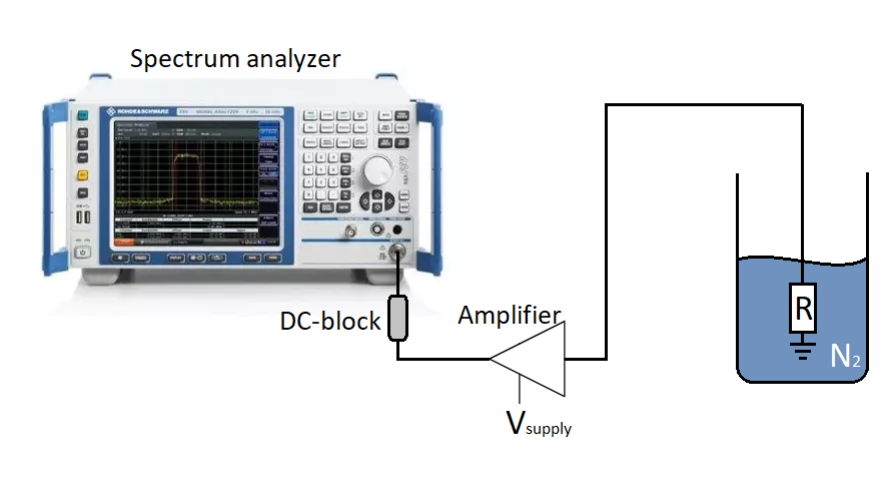
\includegraphics[width=1\linewidth]{PHYS_C0258_Noise_measurements}
	\caption{Complete setup for the liquid nitrogen experiment}
	\label{fig:physc0258noisemeasurements}
\end{figure}
 
 \subsection{Amplifiers}
 
 For our experiment, we use 2 $\qty{20}{\decibel}$ amplifiers connected one after the other. These amplifiers are identical, hence the order does not matter, however, it is quite essential for multi-amplifier setups. For a 2 amplifier setup, the power output is 
 
 \begin{equation}
 	P_{\textrm{out}} = G_1G_2k_B\left(T+T_{N_1}+\tfrac{T_{N_2}}{G_1} \right)\Delta f
 \end{equation}
 
 We can rewrite this equation to get the temperature instead:
 
  \begin{equation}
 	T = \tfrac{P_{\textrm{out}}}{G_1G_2k_B\Delta f} -T_{N_1} -\tfrac{T_{N_2}}{G_1} 
 \end{equation}
 
 As such, the noise temperature for the first amplifier determines most of the noise. The details for our amplifiers are given below:
 
\begin{figure}[H]
	\includegraphics[width=1\linewidth]{"noise of minicircuits amplifier chain"}
	\caption{Schematic diagram of the amplifier setup}
	\label{fig:noise-of-minicircuits-amplifier-chain}
\end{figure}
\section{Results}
\hypertarget{noise-floor-sweep-from-0-to-12-ghz-without-load-or-amplifier}{%
	\subsection{\texorpdfstring{Noise floor sweep from \(0\) to \(12\) GHz
			without load or
			amplifier}{Noise floor sweep from 0 to 12 GHz without load or amplifier}}\label{noise-floor-sweep-from-0-to-12-ghz-without-load-or-amplifier}}

\begin{figure}[H]
	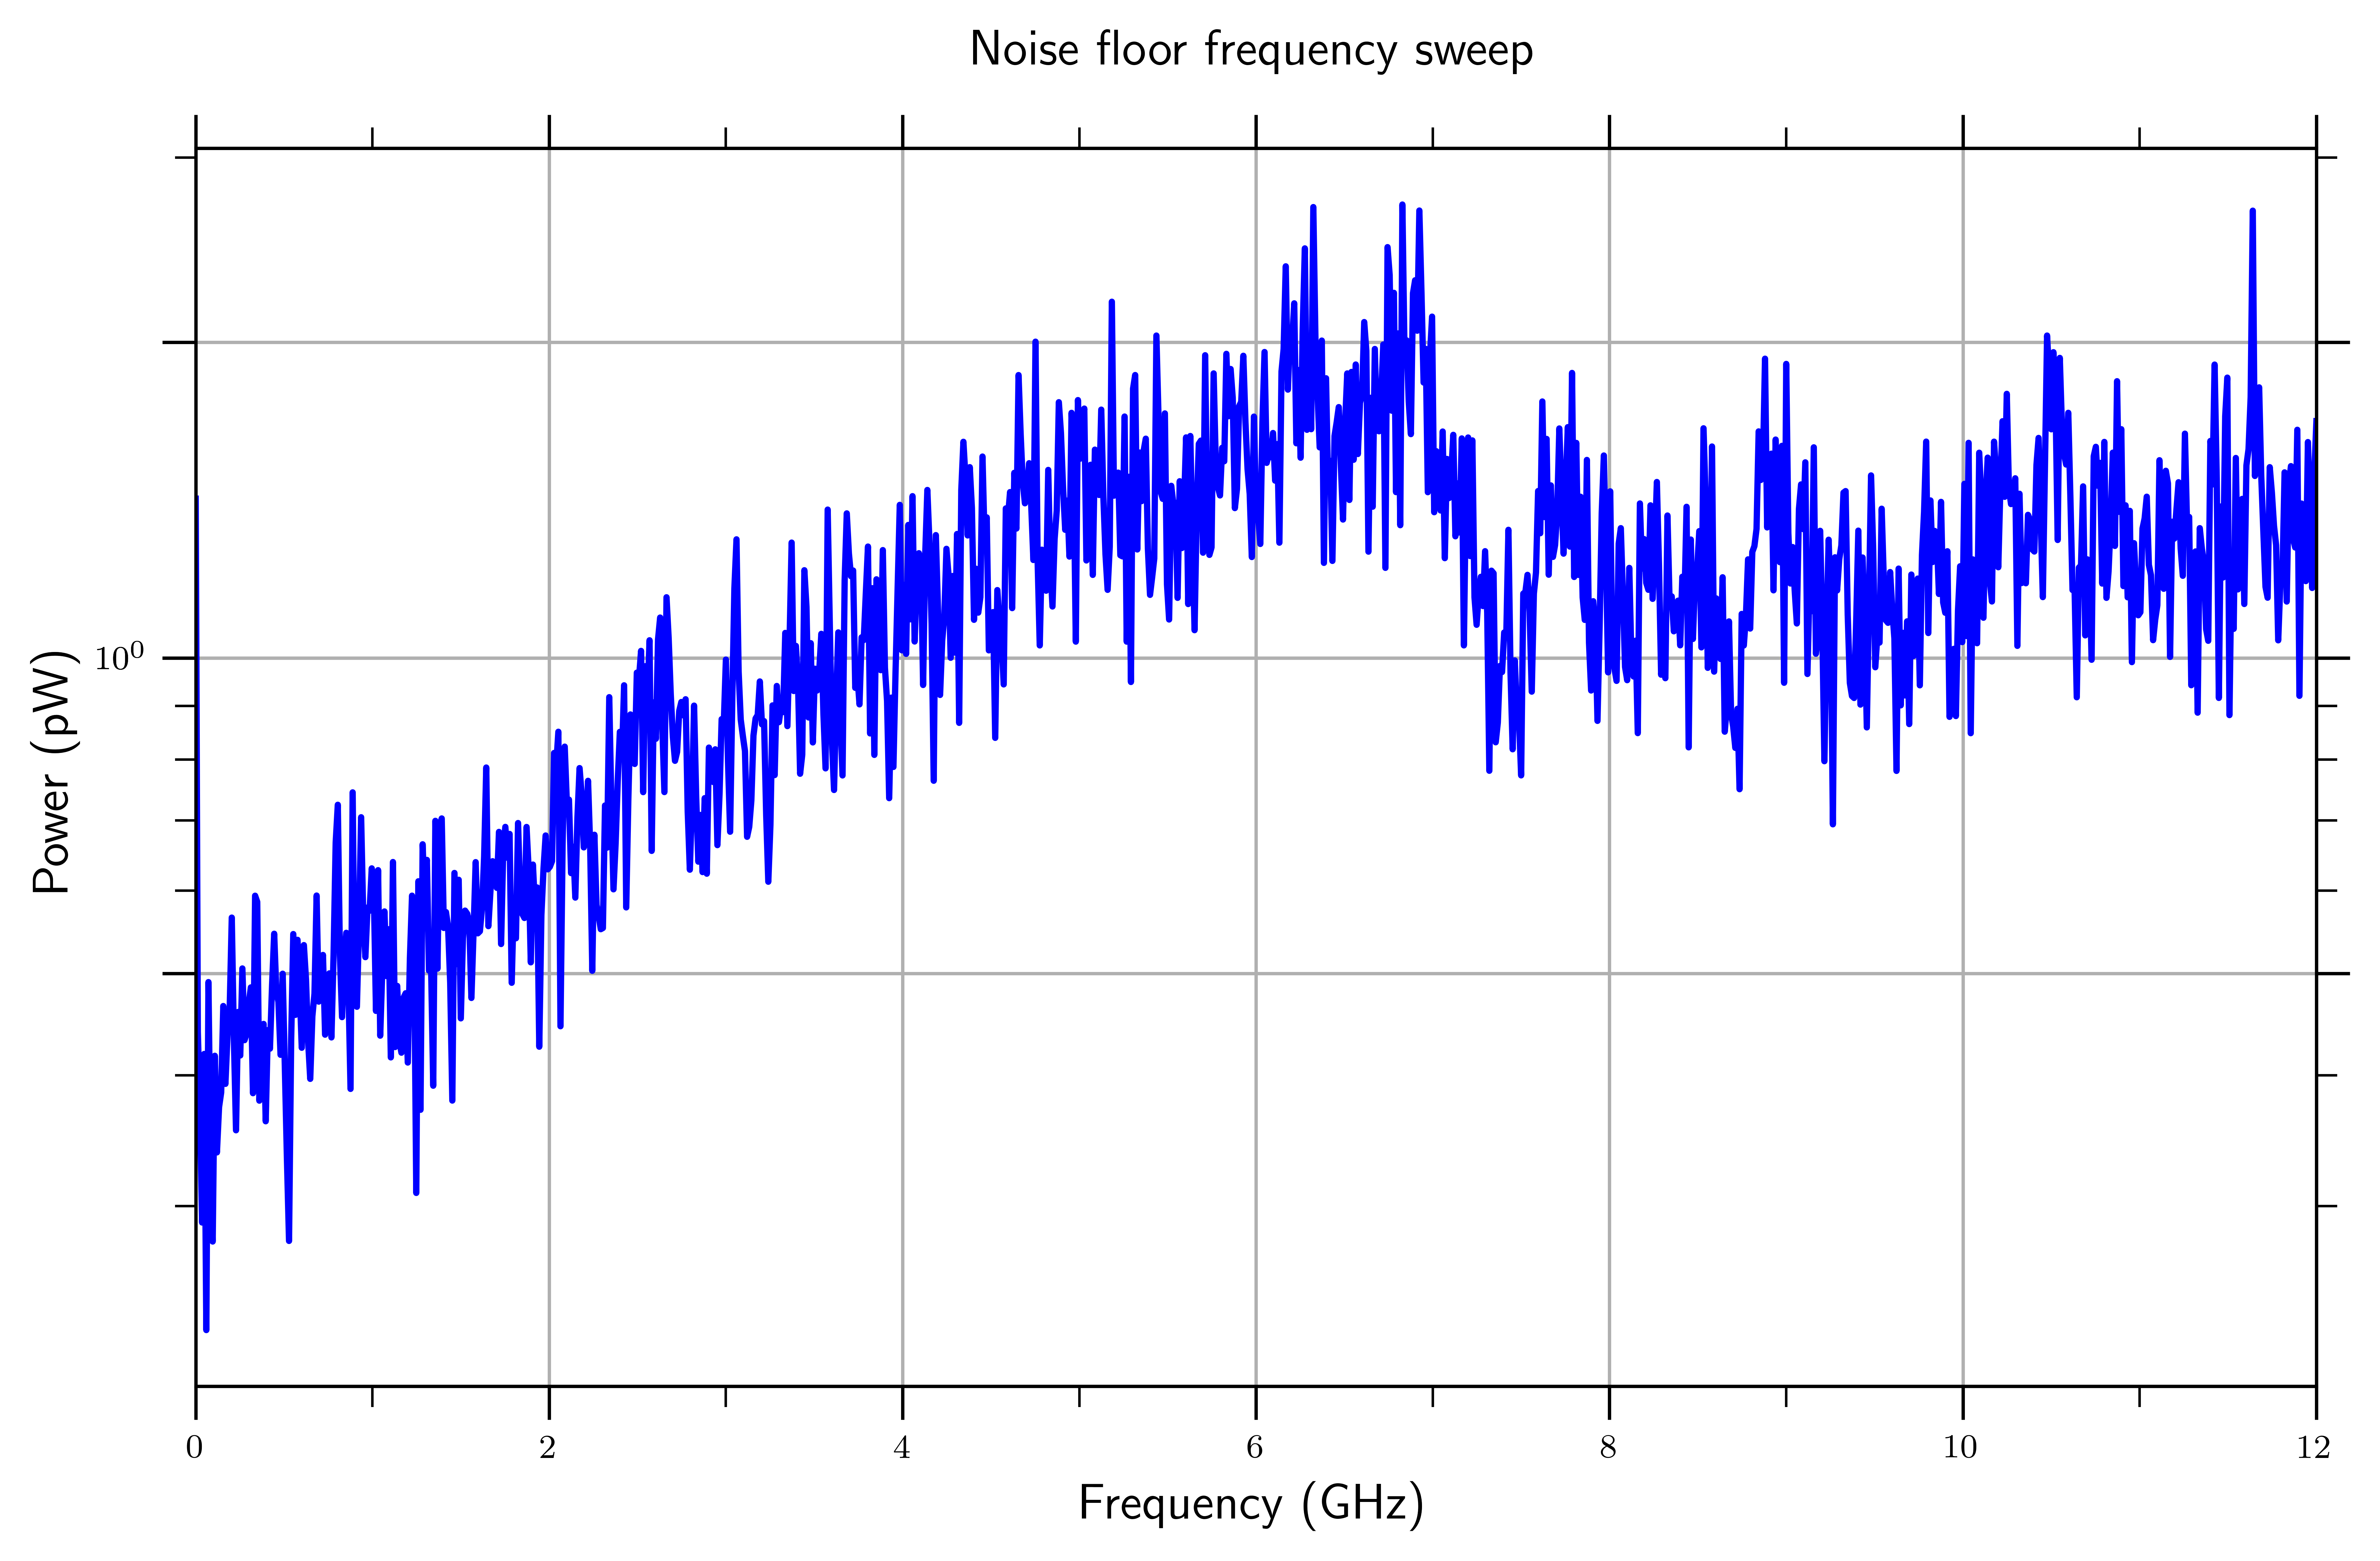
\includegraphics[width=1\linewidth]{Plots/noise_floor_sweep}
	\caption[Noise floor frequency sweep]{}
	\label{fig:noisefloorsweep}
\end{figure}

 

\hypertarget{noise-floor-measurements-at-6-ghz-without-load-or-amplifier}{%
	\subsection{\texorpdfstring{Noise floor measurements at \(6\) GHz without
			load or
			amplifier}{Noise floor measurements at 6 GHz without load or amplifier}}\label{noise-floor-measurements-at-6-ghz-without-load-or-amplifier}}

 

\hypertarget{raw-data-with-the-mean-highlighted}{%
	\subsubsection{Raw data with the mean
		highlighted}\label{raw-data-with-the-mean-highlighted_1}}

\begin{figure}[H]
	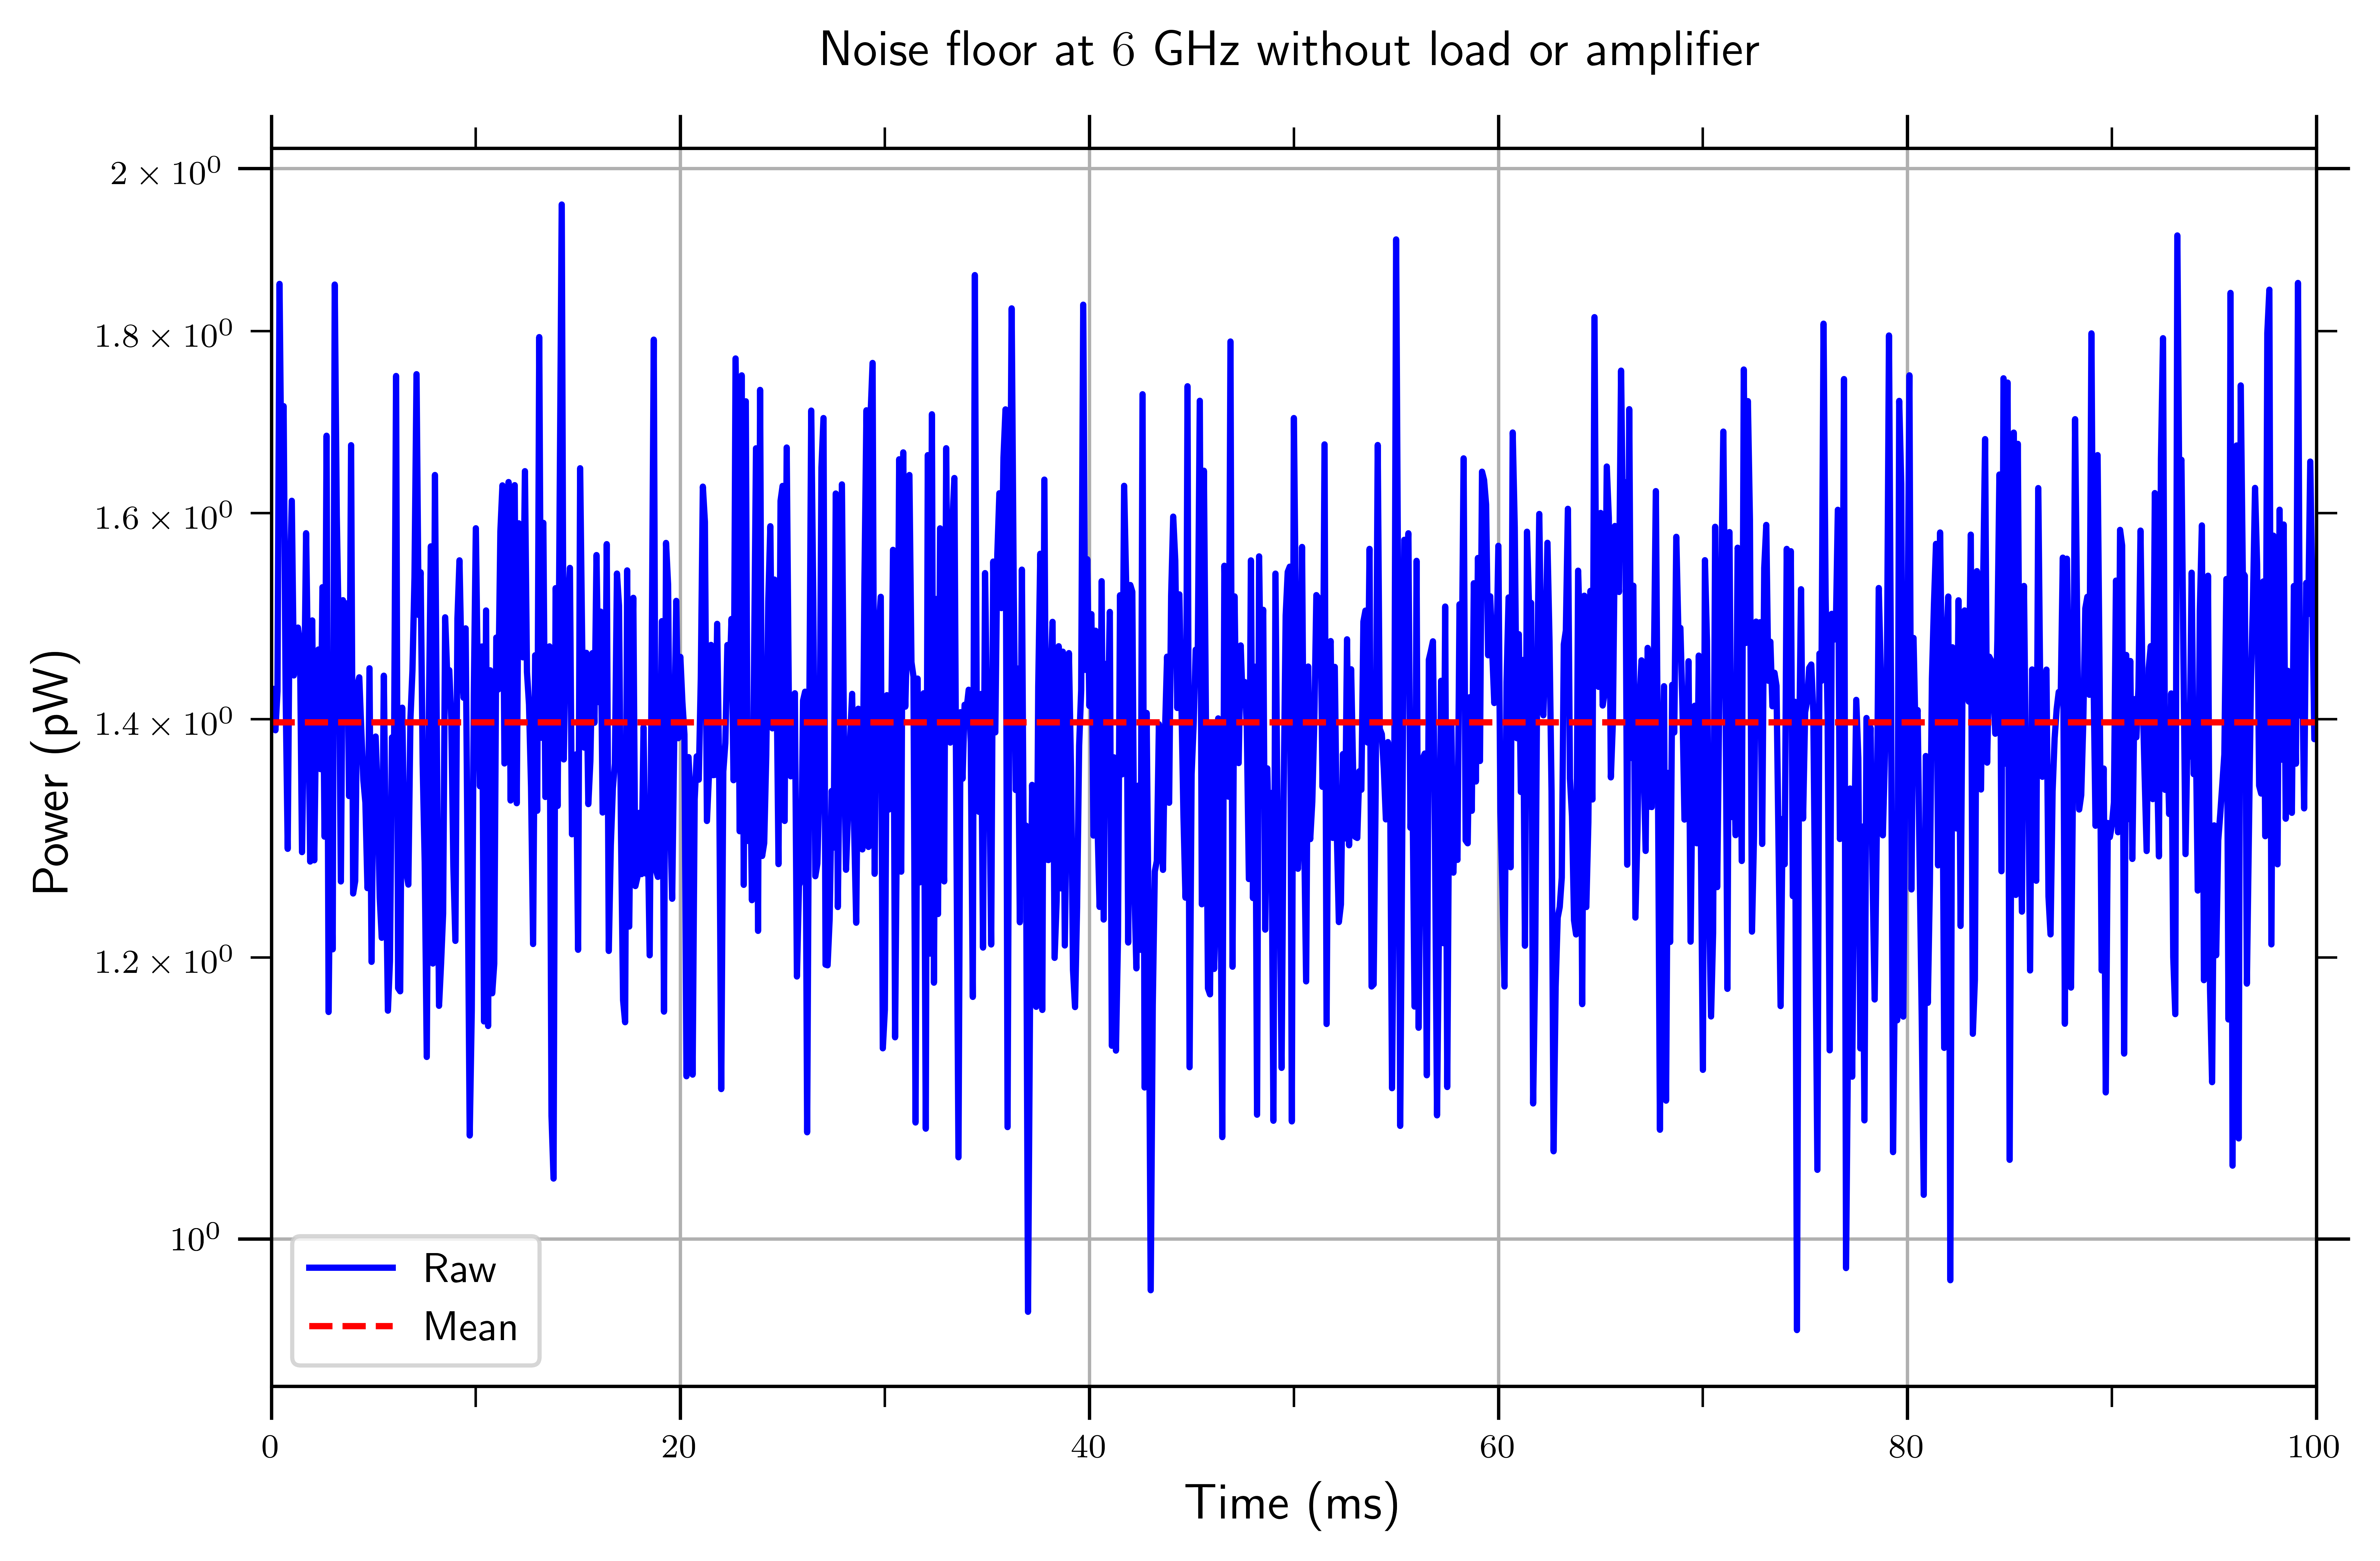
\includegraphics[width=1\linewidth]{Plots/noise_floor_6_GHz}
	\caption[Noise floor at 6 GHz]{}
	\label{fig:noisefloor6ghz}
\end{figure}



\hypertarget{noise-analysis}{%
	\subsubsection{Noise analysis}\label{noise-analysis_1}}

	The actual average power is $\qty{1.397}{\pico\watt}$.
	The noise level calculated via root mean square is $\qty{1.407}{\pico\watt}$.
	The noise level calculated via peak-to-peak is $\qty{1.011}{\pico\watt}$.
	
	The signal-to-noise ratio calculated via root mean square is $0.9930$.
	The signal-to-noise ratio calculated via peak-to-peak is $1.382$.


\hypertarget{noise-measurements-at-6-ghz-with-a-50-omega-load-but-no-amplifier}{%
	\subsection{\texorpdfstring{Noise measurements at \(6\) GHz with a
			\(50 \Omega\) load but no
			amplifier}{Noise measurements at 6 GHz with a 50 \textbackslash Omega load but no amplifier}}\label{noise-measurements-at-6-ghz-with-a-50-omega-load-but-no-amplifier}}



\hypertarget{raw-data-with-the-mean-highlighted}{%
	\subsubsection{Raw data with the mean
		highlighted}\label{raw-data-with-the-mean-highlighted-6}}

\begin{figure}[H]
	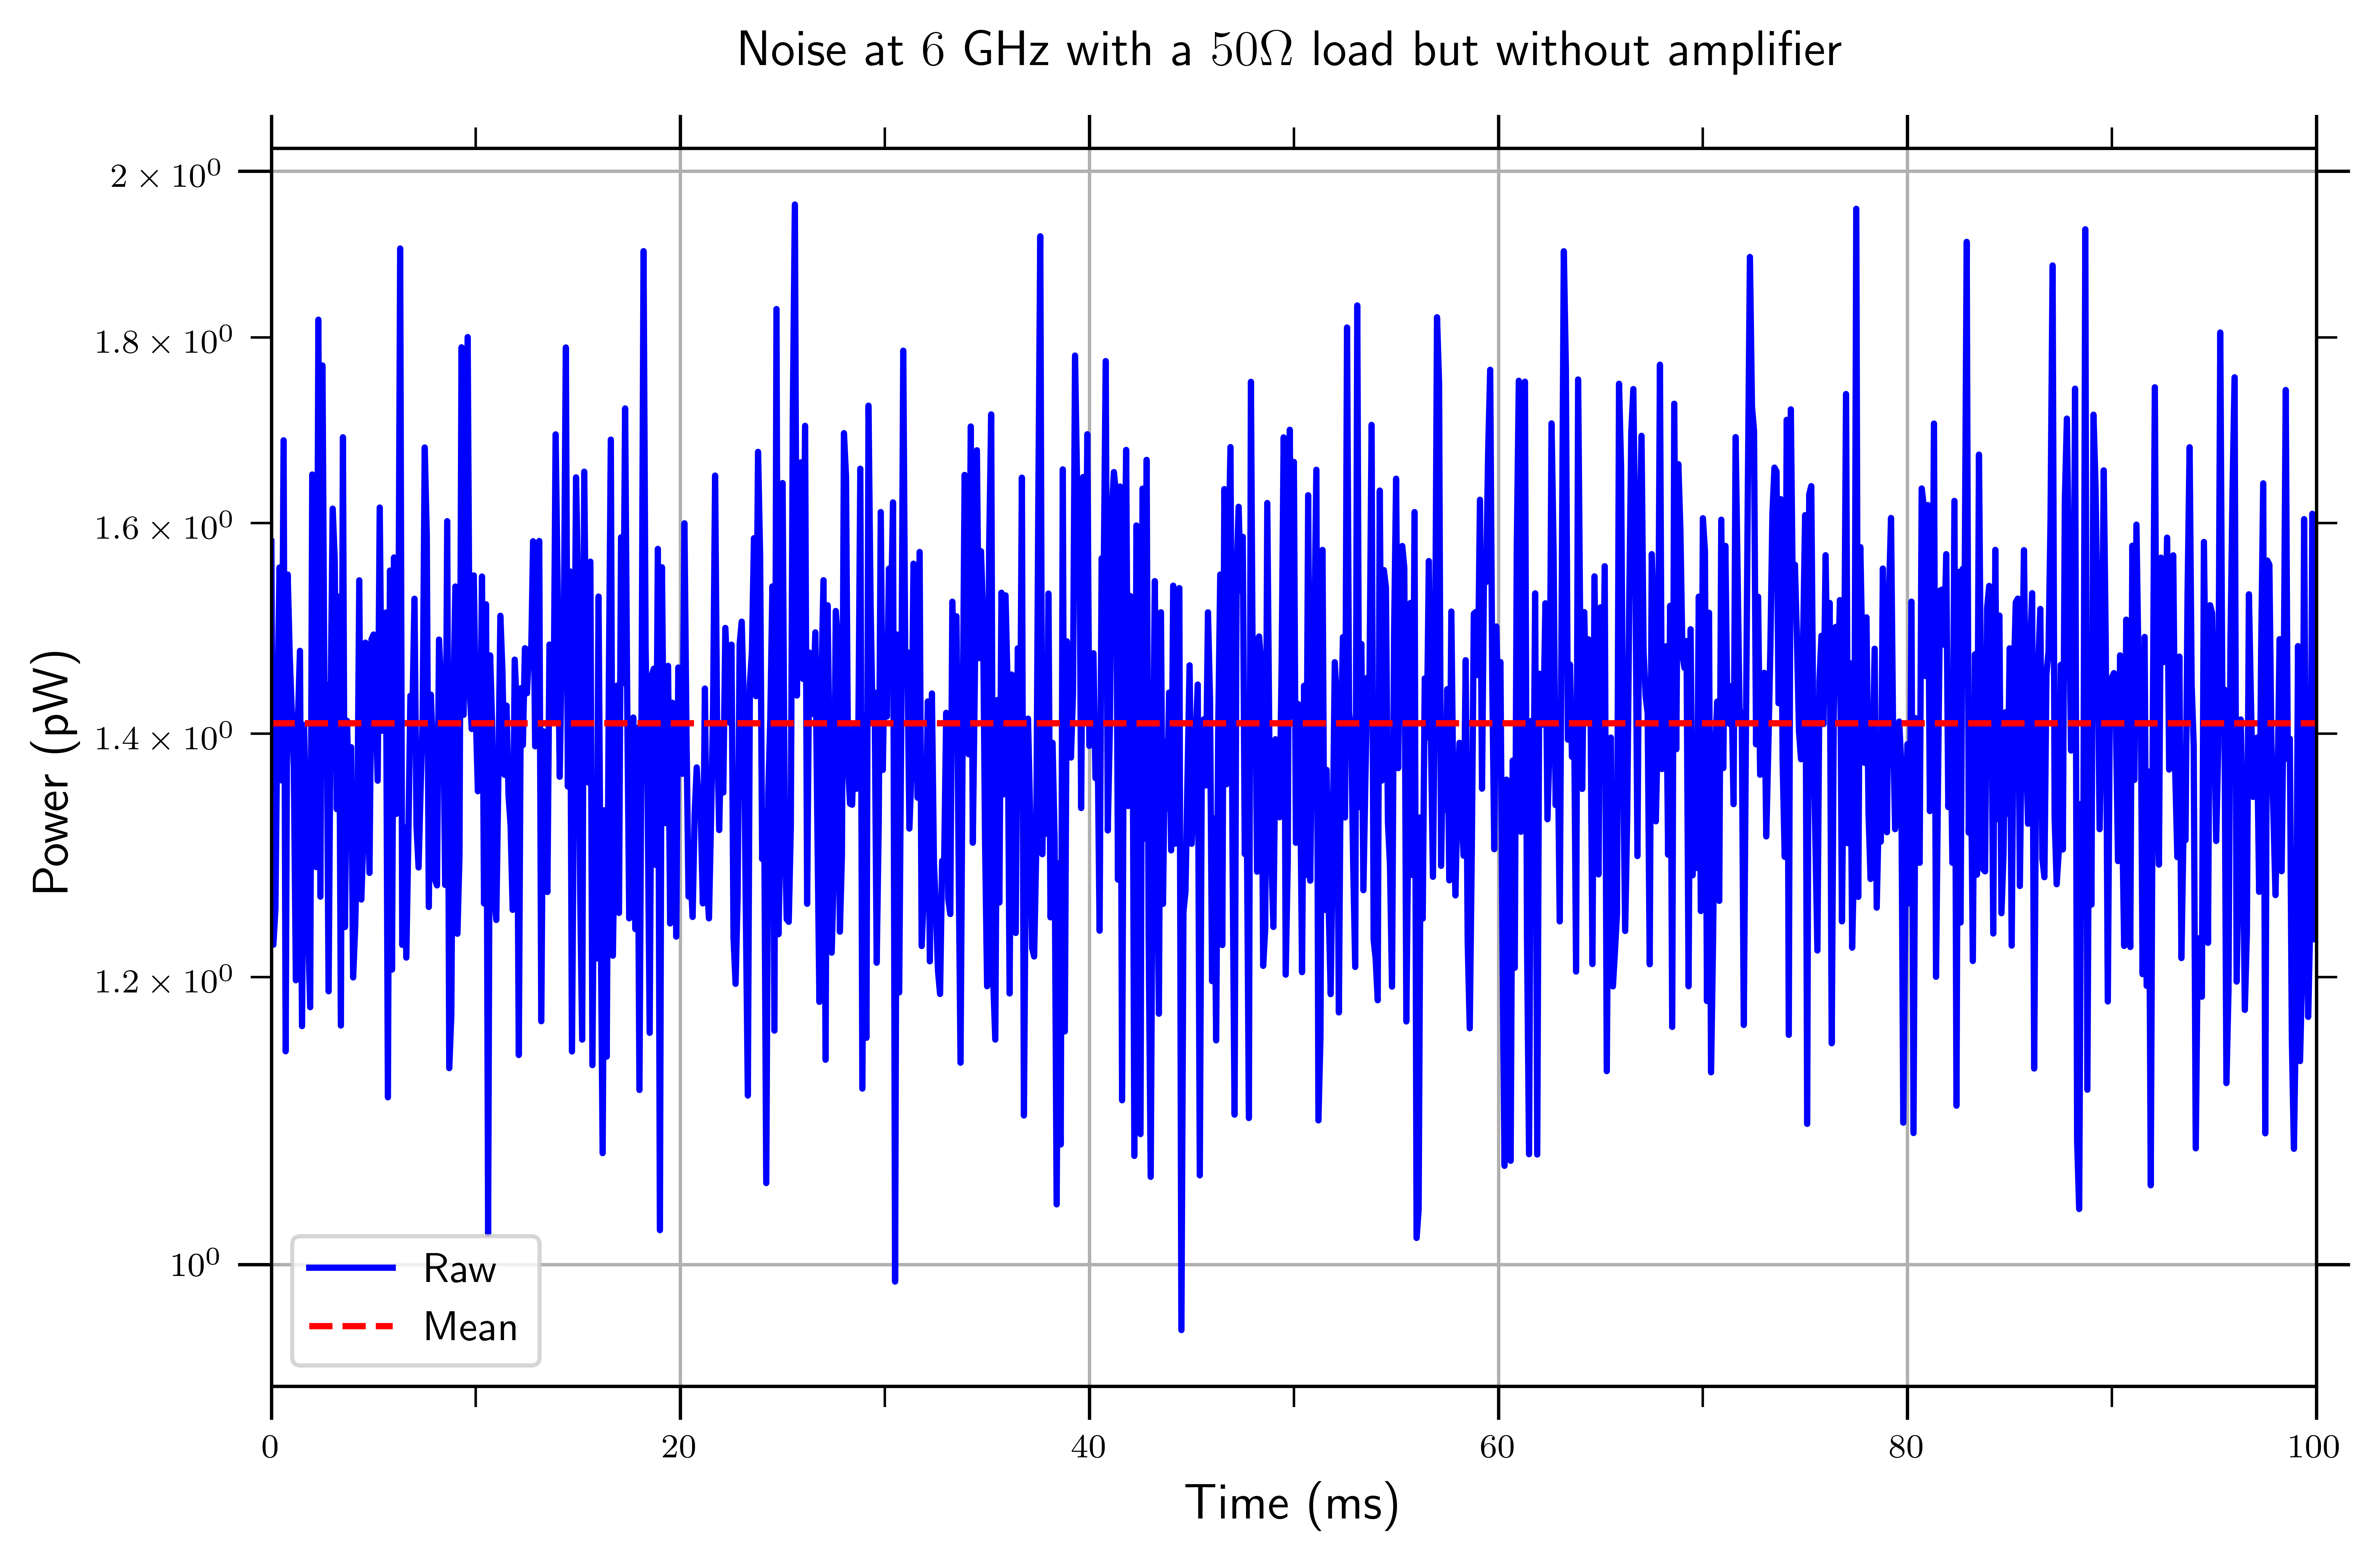
\includegraphics[width=1\linewidth]{Plots/noise_floor_6_GHz_50ohm}
	\caption[Noise measurements at 6 GHz with a 50 Ohm load]{}
	\label{fig:noisefloor6ghz50ohm}
\end{figure}

 

\hypertarget{noise-analysis}{%
	\subsubsection{Noise analysis}\label{noise-analysis_2}}

	The expected power is $k_B T\Delta f = k_B \times \qty{298}{\kelvin} \times \qty{2}{\mega\hertz} \approx \qty{8.229}{\femto\watt}$.
	
	However, the average power is $\qty{1.410}{\pico\watt}$.
	The noise level calculated via root mean square is $\qty{1.420}{\pico\watt}$.
	The noise level calculated via peak-to-peak is $\qty{0.9987}{\pico\watt}$.
	
	The signal-to-noise ratio calculated via root mean square is $0.9929$.
	The signal-to-noise ratio calculated via peak-to-peak is $1.411$.

\hypertarget{noise-measurements-at-6-ghz-with-an-amplifier-but-no-load}{%
	\subsection{\texorpdfstring{Noise measurements at \(6\) GHz with an
			amplifier but no
			load}{Noise measurements at 6 GHz with an amplifier but no load}}\label{noise-measurements-at-6-ghz-with-an-amplifier-but-no-load}}


\hypertarget{raw-data-with-the-mean-highlighted}{%
	\subsubsection{Raw data with the mean
		highlighted}\label{raw-data-with-the-mean-highlighted_2}}

\begin{figure}[H]
	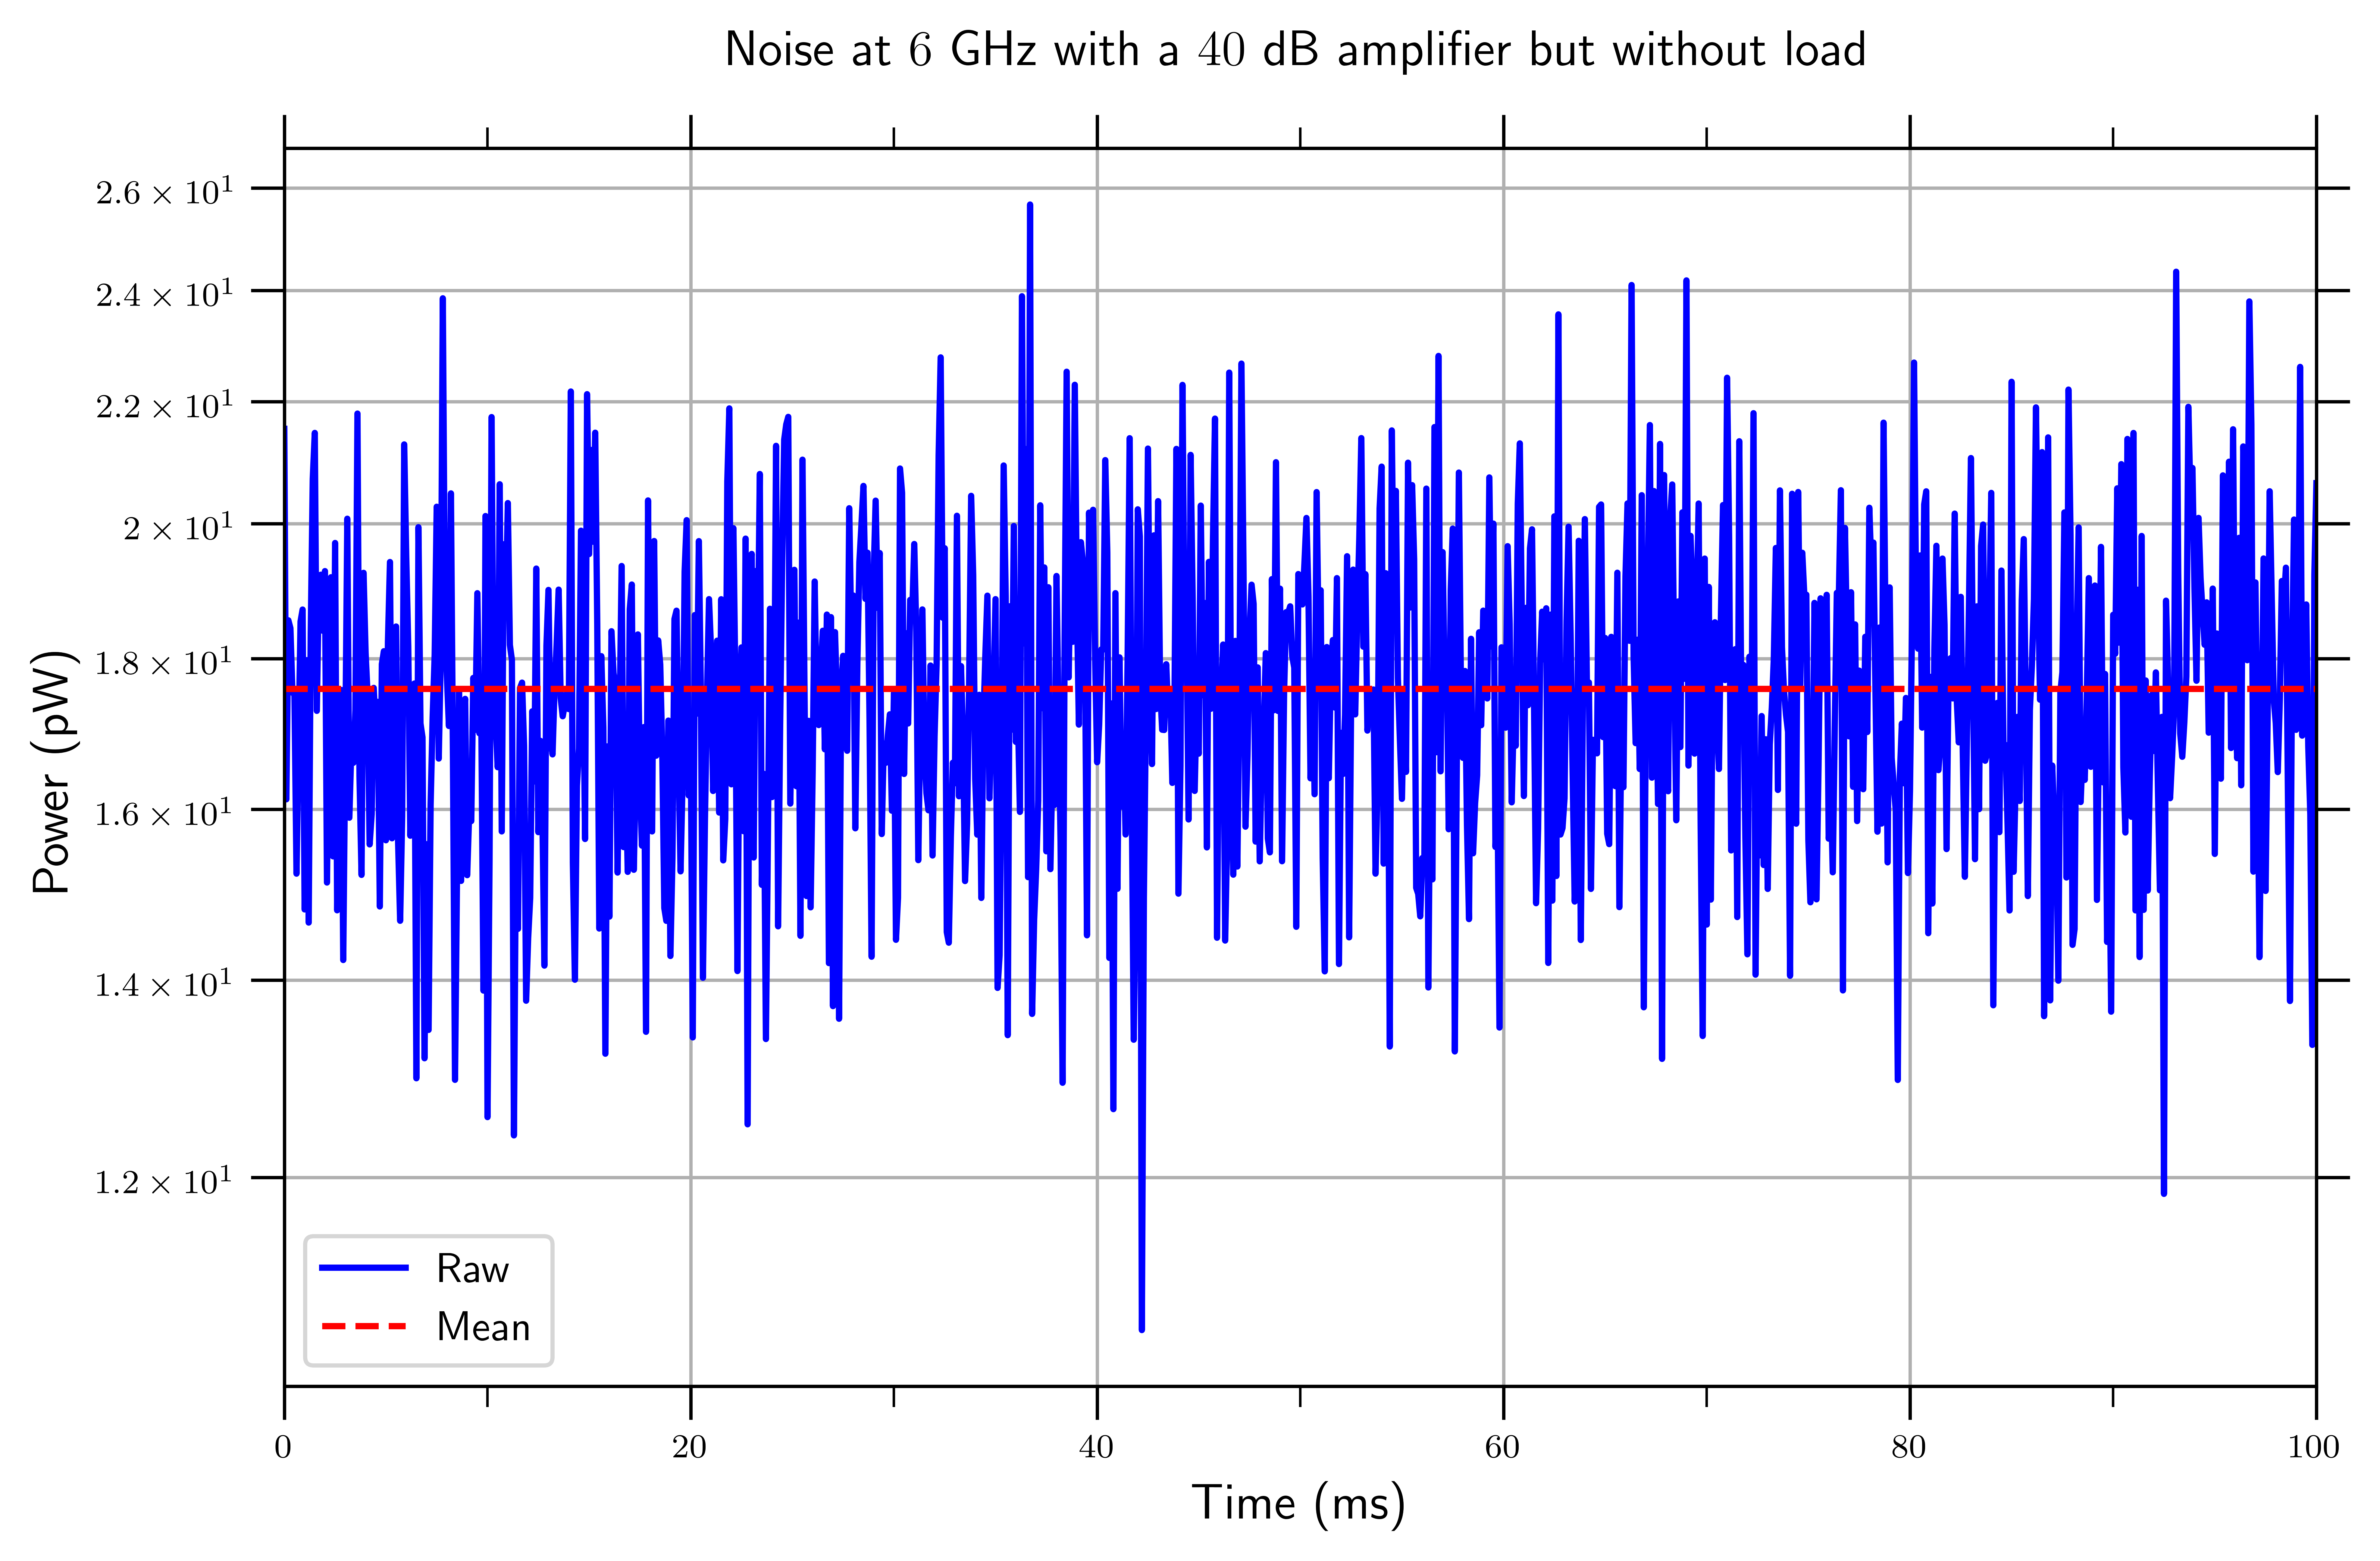
\includegraphics[width=1\linewidth]{Plots/noise_floor_6_GHz_amplif}
	\caption{Noise measurements at 6 GHz with an amplifier}
	\label{fig:noisefloor6ghzamplif}
\end{figure}
 

\hypertarget{noise-analysis}{%
	\subsubsection{Noise analysis}\label{noise-analysis_3}}


	The average power is $\qty{17.58}{\pico\watt}$.
	The noise level calculated via root mean square is $\qty{17.71}{\pico\watt}$.
	The noise level calculated via peak-to-peak is $\qty{15.01}{\pico\watt}$.
	
	The signal-to-noise ratio calculated via root mean square is $0.9927$.
	The signal-to-noise ratio calculated via peak-to-peak is $1.171$.


\hypertarget{noise-measurements-at-6-ghz-with-a-40-db-amplifier-and-a-50-omega-load-at-293k}{%
	\subsection{Noise measurements at $\qty{6}{\giga\hertz}$ with a $\qty{40}{\decibel}$ amplifier and a $\qty{50}{\ohm}$ load at $\qty{293}{\kelvin}$}\label{noise-measurements-at-6-ghz-with-a-40-db-amplifier-and-a-50-omega-load-at-293k}}

 

\hypertarget{raw-data-with-the-mean-highlighted}{%
	\subsubsection{Raw data with the mean
		highlighted}\label{raw-data-with-the-mean-highlighted_3}}

\begin{figure}[H]
	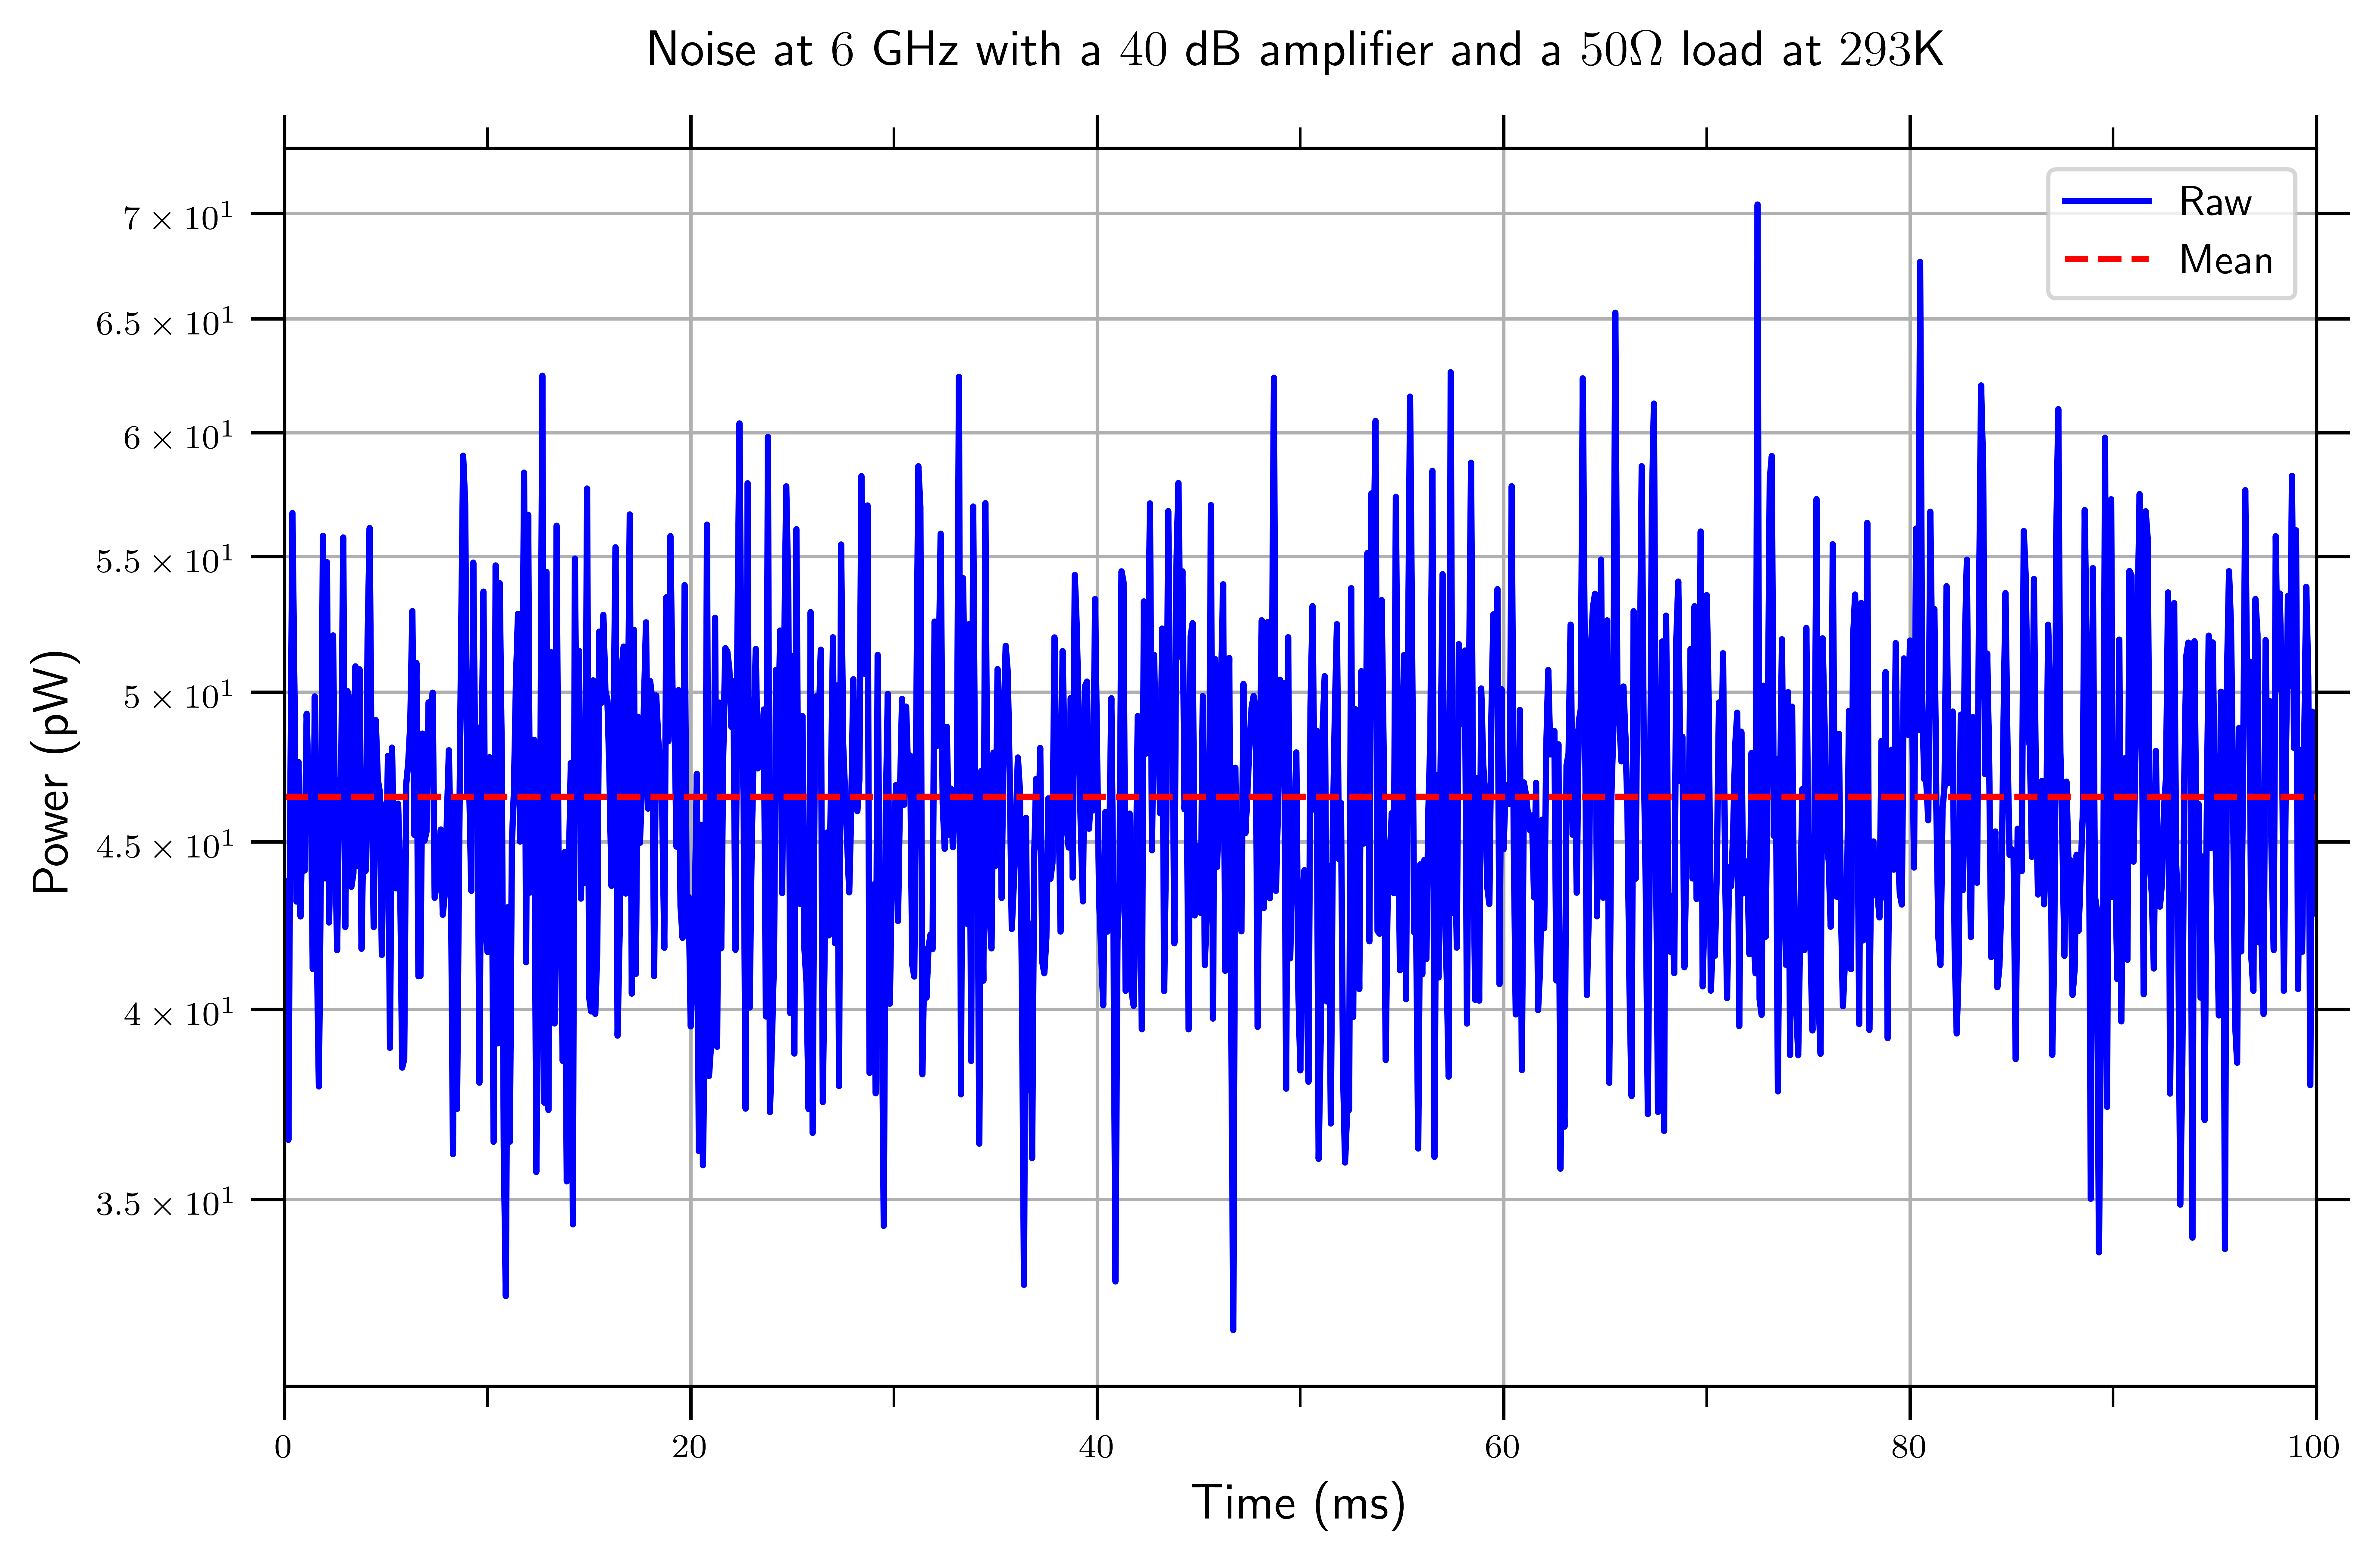
\includegraphics[width=1\linewidth]{Plots/noise_floor_6_GHz_amplif_50ohm_rt}
	\caption{Noise measurements at $\qty{6}{\giga\hertz}$ with a $\qty{40}{\decibel}$ amplifier and a $\qty{50}{\ohm}$ load at $\qty{293}{\kelvin}$}
	\label{fig:noisefloor6ghzamplif50ohmrt}
\end{figure}


\hypertarget{noise-analysis}{%
	\subsubsection{Noise analysis}\label{noise-analysis_4}}



	The average power is $\qty{46.45}{\pico\watt}$.
	The noise level calculated via root mean square is $\qty{46.79}{\pico\watt}$.
	The noise level calculated via peak-to-peak is $\qty{38.51}{\pico\watt}$.
	
	The signal-to-noise ratio calculated via root mean square is $0.9927$.
	The signal-to-noise ratio calculated via peak-to-peak is $1.206$.
	
\subsection{Noise measurements at $\qty{6}{\giga\hertz}$ with a $\qty{40}{\decibel}$ amplifier and a $\qty{50}{\ohm}$ load at $\qty{77}{\kelvin}$}

\hypertarget{raw-data-with-the-mean-highlighted}{%
	\subsubsection{Raw data with the mean
		highlighted}\label{raw-data-with-the-mean-highlighted_7}}

\begin{figure}[H]
	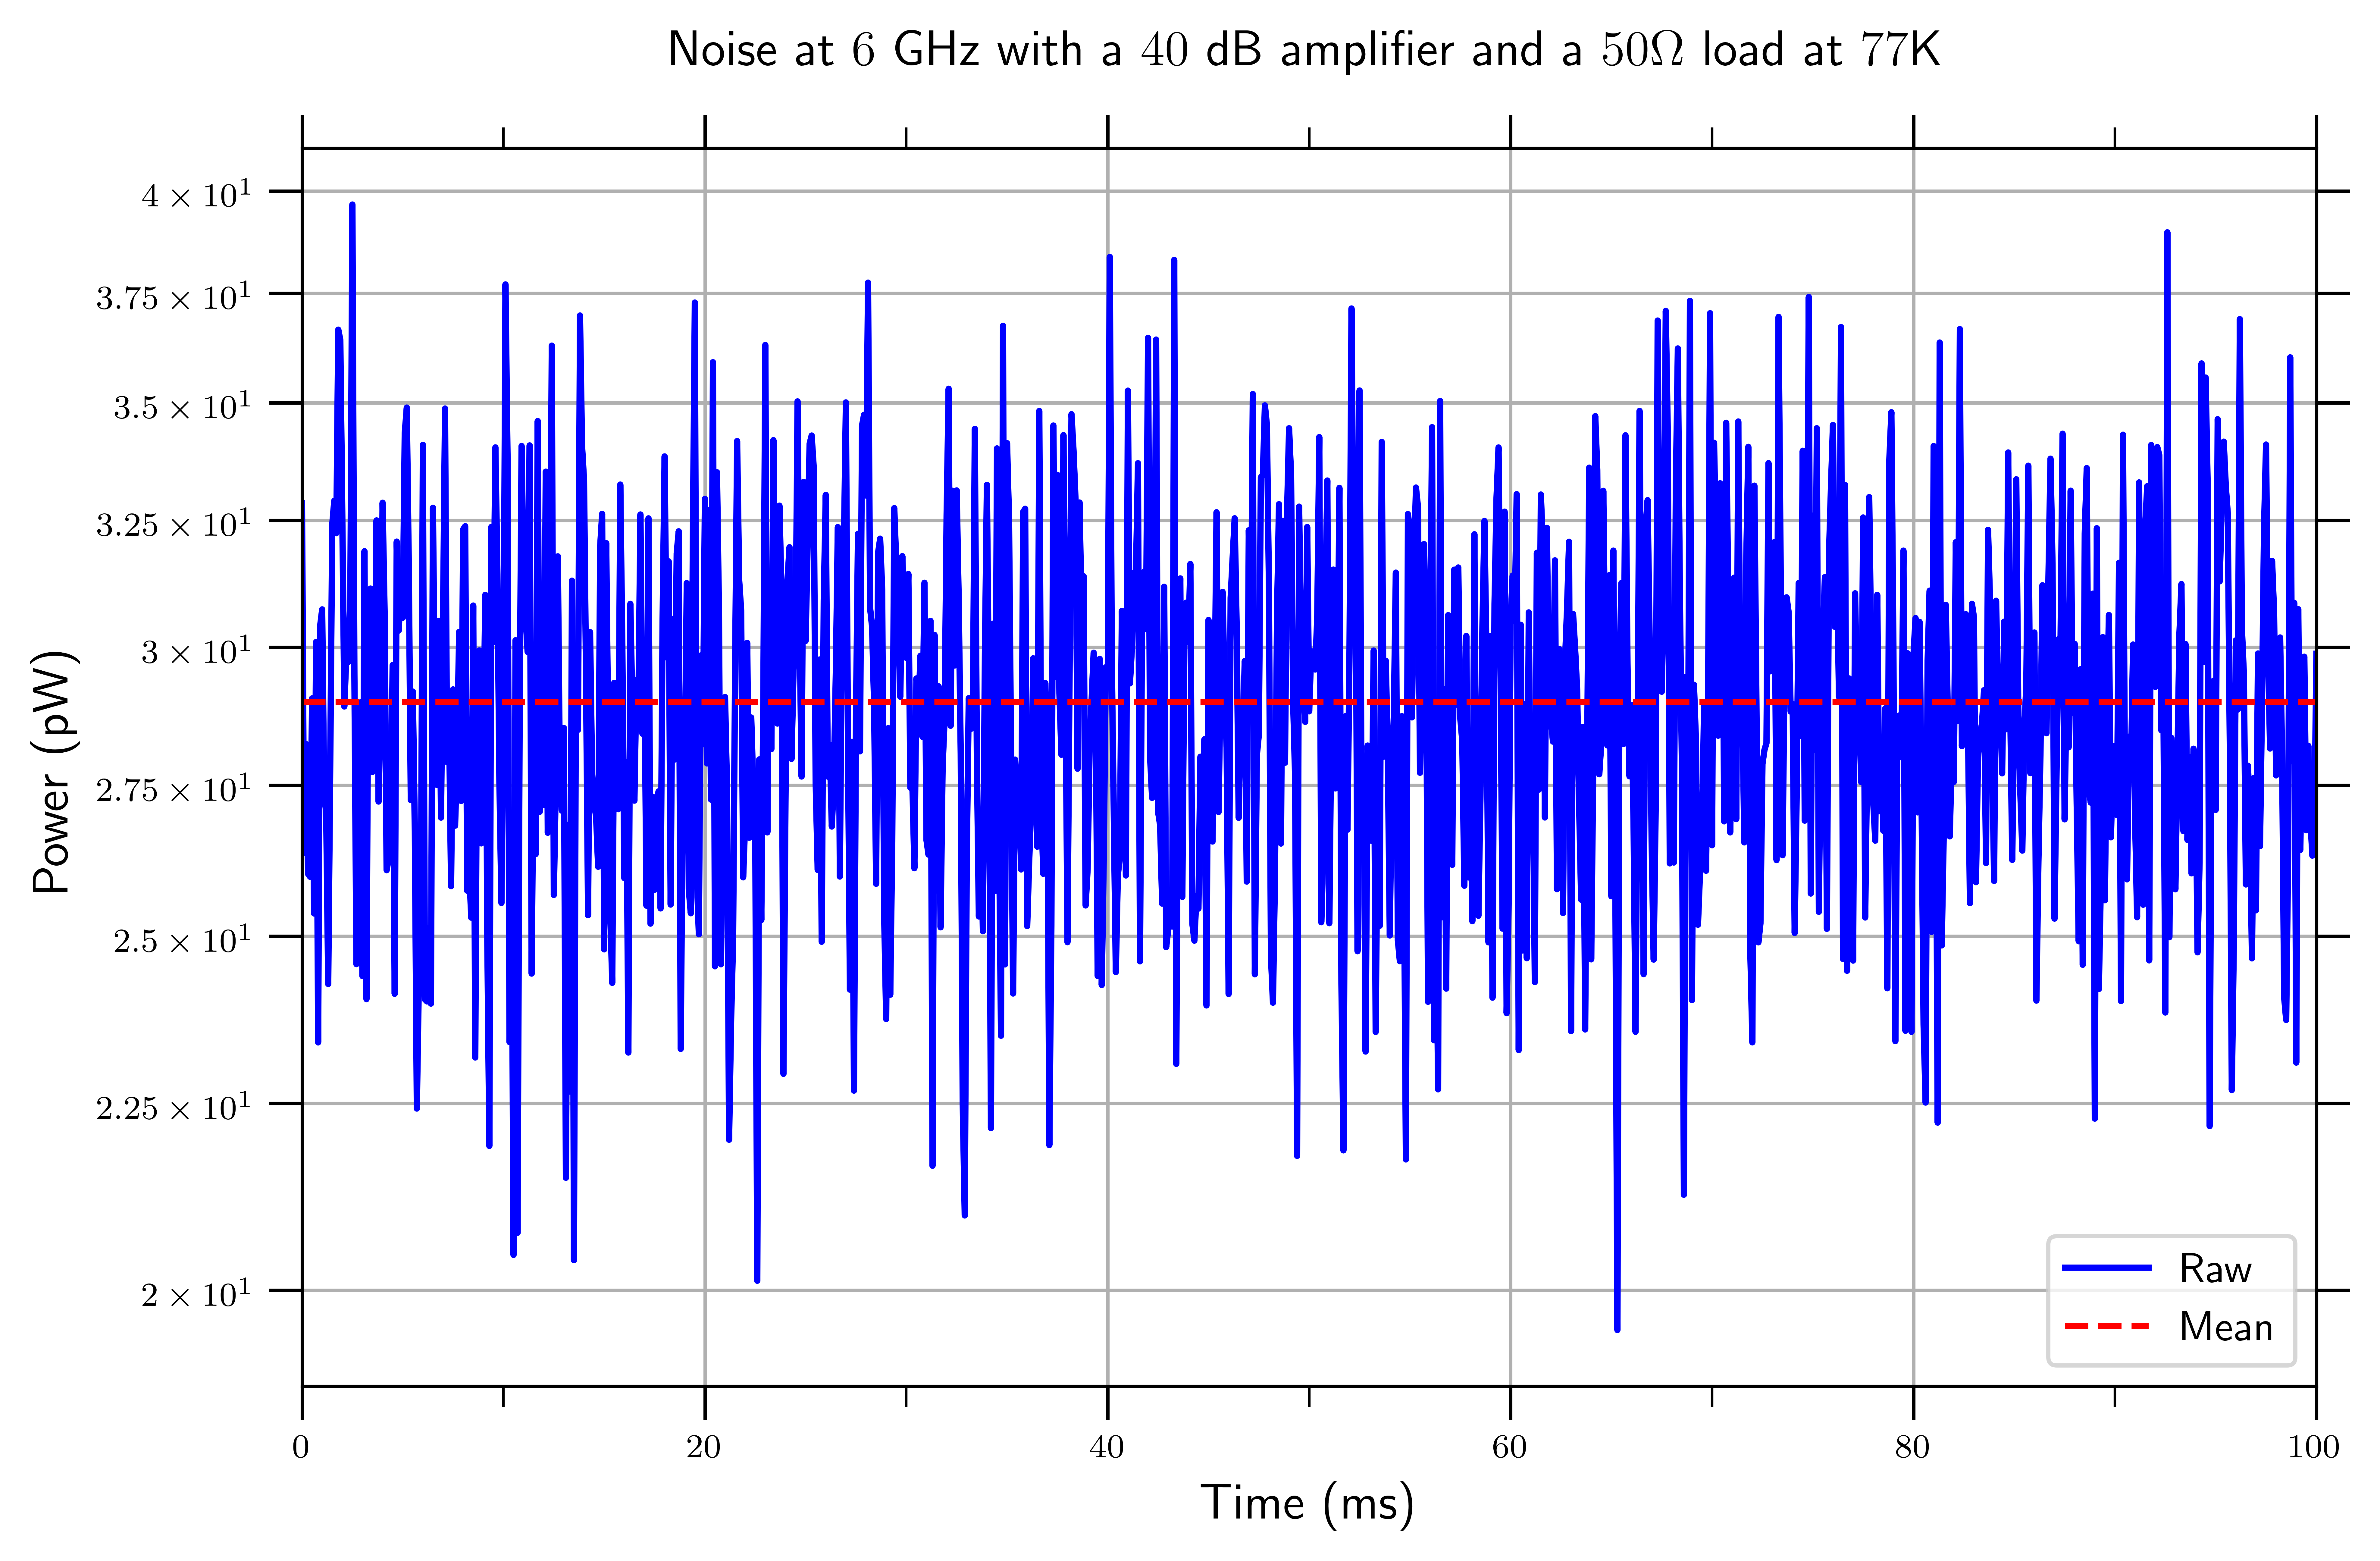
\includegraphics[width=1\linewidth]{Plots/noise_floor_6_GHz_amplif_50ohm_lt}
	\caption{Noise measurements at $\qty{6}{\giga\hertz}$ with a $\qty{40}{\decibel}$ amplifier and a $\qty{50}{\ohm}$ load at $\qty{77}{\kelvin}$}
	\label{fig:noisefloor6ghzamplif50ohmlt}
\end{figure}

 

\hypertarget{noise-analysis}{%
	\subsubsection{Noise analysis}\label{noise-analysis_7}}


	The average power is $\qty{28.99}{\pico\watt}$.
	The noise level calculated via root mean square is $\qty{29.18}{\pico\watt}$.
	The noise level calculated via peak-to-peak is $\qty{20.15}{\pico\watt}$.
	
	The signal-to-noise ratio calculated via root mean square is $0.9932$.
	The signal-to-noise ratio calculated via peak-to-peak is $1.438$.

\section{Conclusion}
We get an average power of  $\qty{28.99}{\pico\watt}$. As such, we can back estimate the temperature using equation $3$.  This gives us a value of 
\section{References}
\printbibliography
\end{document}